\chapter{Corriente alterna monofásica}\label{chap.ca_mono}
 	
 	\section{Formas de onda periódicas}
 	
 		En los circuitos eléctricos, las funciones de excitación y respuesta son tensiones
	e intensidades que varían con el tiempo:
	\begin{align*}
		u&=u(t)\\
		i&=i(t)
	\end{align*}
	Estas funciones pueden representarse de forma gráfica o analítica. En ambos
	casos, esa relación funcional se conoce mediante el nombre de \textbf{forma de onda}. Las formas de onda pueden clasificarse según (de manera análoga a lo indicado en la Sección~\ref{sec.cc-ca}):
	\begin{itemize}
		\item \textbf{Signo de la magnitud}:
		\begin{itemize}
			\item \textbf{Unidireccionales}: la magnitud que la representa siempre tiene una única polaridad (signo constante, aunque el valor puede ser constante o variable)
			\item \textbf{Bidireccionales}: la magnitud toma valores positivos y negativos (signo variable con el tiempo)
		\end{itemize}
		\item \textbf{Repetición del valor de la magnitud}:
		\begin{itemize}
			\item \textbf{Periódicas}: el valor de la magnitud se repite de forma regular
			\item \textbf{No periódicas}: el valor de la magnitud varía de forma arbitraria con el tiempo
		\end{itemize}
	\end{itemize}

	Cuando se trabaje con \textbf{corriente alterna}, siempre se usarán \textbf{funciones de onda periódicas}, generalmente sinusoidales. Las formas de onda periódicas son aquellas que se repiten a intervalos iguales de tiempo y en el mismo orden, siguiendo la expresión:
	\begin{equation*}
		y(t)=y(t+T)=y(t+n\cdot T)
	\end{equation*}
	
	Existen una serie de definiciones y valores de interés para las ondas periódicas:
	\begin{itemize}
		\item \textbf{Período ($T$)}: intervalo de tiempo mínimo a partir del cual se repite la forma de onda [s]
		\item \textbf{Frecuencia ($f$)}: número de veces que se repite la onda por unidad de tiempo [Hz]:
		\begin{equation*}
			f = \dfrac{1}{T}
		\end{equation*}
		\begin{remark}
		    La unidad [Hz] se escribe en mayúsculas en honor a Heinrich Rudolf Hertz, físico alemán del siglo XIX que descubrió el efecto fotoeléctrico, la propagación de las ondas electromagnéticas y las formas para producirlas y detectarlas.
		\end{remark}
		\item \textbf{Valor instantáneo}: valor $y(t)$ que toma la forma de onda en un instante de tiempo dado
		\item \textbf{Valores de pico ($Y_{max}$, $Y_{min}$)}: valores máximo y mínimo que toma la forma de onda en un periodo:
		\begin{equation*}
			Y_{max} = \max(f(t)); \qquad Y_{min} = \min(f(t))
		\end{equation*}
		\item \textbf{Valor pico a pico ($Y_{PP}$)}: se corresponde con la diferencia (en valor absoluto) entre los valores de pico considerados con signo: 
		\begin{equation*}
			Y_{PP}=|Y_{max} - Y_{min}|
		\end{equation*}
		\item \textbf{Valor medio ($Y_m$)}: en un intervalo ($t_1,t_2$), corresponde con la media aritmética de los valores instantáneos que toma la función en dicho intervalo:
		\begin{equation*}
			Y_m=\dfrac{1}{t_2-t_1}\cdot\int_{t_1}^{t_2}y(t)\, dt
		\end{equation*}
		En una onda periódica, se calcula para un intervalo de tiempo igual a un periodo: 
		\begin{equation}\label{eq.valor_medio}
			\boxed{Y_m=\frac{1}{T}\int_{a}^{a+T}y(t)\, dt}
		\end{equation}
		\begin{remark}
			En caso de que el valor medio sea nulo en un periodo, el cálculo se realiza en un semi-periodo ($T/2$) o en un cuarto de periodo ($T/4$)
		\end{remark}
		\item \textbf{Valor eficaz ($Y_{ef}$)}: es la raíz cuadrada de la media de los cuadrados de los valores que toma la función en un intervalo:
		\begin{equation*}
			Y_{ef}=\sqrt{\dfrac{1}{t_2-t_1}\cdot\int_{t_1}^{t_2}y^2(t)\, dt}
		\end{equation*}
		Si es periódica: 
		\begin{equation}\label{eq.valor_eficaz}
			\boxed{Y_{ef} = \sqrt{\frac{1}{T}\cdot\int_{a}^{a+T}y^{2}(t)\, dt}}
		\end{equation}
		\item \textbf{Factor de amplitud ($FA$)}: es el cociente entre el valor máximo y el valor eficaz de una onda:
		\begin{equation*}
			FA = \dfrac{Y_{max}}{Y_{ef}}
		\end{equation*}
		\item \textbf{Factor de forma ($FF$)}: es el cociente entre el valor eficaz y el valor medio:
		\begin{equation*}
			FF = \dfrac{Y_{ef}}{Y_{m}}
		\end{equation*}
		\begin{remark}
			Si el valor medio fuese nulo en un período, se toma el de un semiperíodo
		\end{remark}
	\end{itemize}
	
	\begin{example}\label{ex.forma_onda}
	    \textbf{Hallar el valor medio y eficaz de la onda periódica de la Figura~\ref{fig.forma_onda}.}
	    \begin{figure}[H]
	        \centering
	        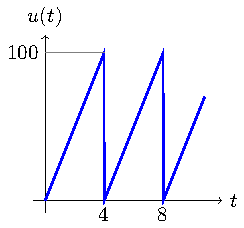
\includegraphics{../figs/ejemplo_forma_onda.pdf}
	        \caption{Ejemplo~\ref{ex.forma_onda}}
	        \label{fig.forma_onda}
	    \end{figure}
	    
	    La onda es una función periódica, de periodo $T=4$ s, para la cual, en el intervalo $[0,4]$ s, la función se expresa como:
	    \begin{equation*}
	        u(t)=\dfrac{100}{4}\,t=25\,t\quad (0\leq t\leq 4\,\text{s})
	    \end{equation*}
	    
	    Se utiliza la expresión~\eqref{eq.valor_medio} para determinar el valor medio: 
	    \begin{equation*}
	        U_m=\dfrac{1}{T}\int_0^T u(t)\,dt=\dfrac{1}{4}\int_0^4 (25\,t)\,dt=\dfrac{1}{4}\,\left[25\,\dfrac{t^2}{2} \right]_0^4={50}
	    \end{equation*}
	    
	    Se utiliza la ecuación~\eqref{eq.valor_eficaz} para el valor eficaz:
	    \begin{align*}
	        U_{ef}&=\sqrt{\frac{1}{T}\cdot\int_{0}^{T}u(t)^{2}\, dt}=\sqrt{\frac{1}{4}\cdot\int_{0}^{4}(25\,t)^{2}\, dt}=\sqrt{\frac{1}{4}\cdot\int_{0}^{4}(625\,t^2)\, dt}=\\
	        &=\sqrt{\frac{1}{4}\, 625\,\left[\dfrac{t^3}{3}\right]_0^4}={57.74}
	    \end{align*}
	\end{example}
	
% 	\begin{example}\label{ex.forma_onda2}
% 	    \textbf{Un condensador de 2 F, inicialmente cargado con una tensión $u_C=-3$ V, es alimentado por un generador de corriente cuya forma de onda es la indicada en la Figura~\ref{fig.forma_onda2}.
% 	    \begin{itemize}
% 	        \item Expresar analíticamente $i(t)$
% 	        \item Encontrar la expresión analítica de $u_C(t)$
% 	    \end{itemize}
% 	    }
% 	    \begin{figure}[H]
% 	        \centering
% 	        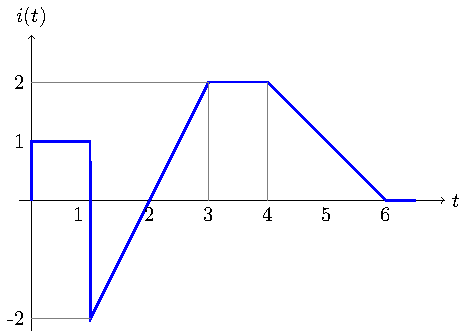
\includegraphics{../figs/ejemplo_ondas2.pdf}
% 	        \caption{Ejemplo~\ref{ex.forma_onda2}}
% 	        \label{fig.forma_onda2}
% 	    \end{figure}
	    
% 	    A partir de la Figura~\ref{fig.forma_onda2} se observa que $i(t)=1$~A para $0<t<1$~s, $i(t)=2$~A para $3<t<4$ e $i(t)=0$ para $t>6$~s. Para los tramos oblicuos se utiliza la expresión general de una recta: 
% 	    \begin{align*}
% 	        i(t)&=\dfrac{2-(-2)}{3-1}(t-2);\quad 1<t<3\\
% 	        i(t)&=\dfrac{0-(-2)}{6-4}(t-6);\quad 4<t<6
% 	    \end{align*}
% 	    Así, la forma analítica para la intensidad $i(t)$ es:
% 	    \begin{equation*}
% 	        i(t)=\begin{cases}
% 	            1\qquad\qquad 0<t<1\\
% 	            2\,t-4 \qquad 1<t<3\\
% 	            2\qquad\qquad 3<t<4\\
% 	            -t+6\qquad 4<t<6\\
% 	            0\qquad\qquad t>6
% 	        \end{cases}
% 	    \end{equation*}
	    
% 	    Para la expresión analítica de $u_C(t)$, hay que utilizar la ecuación propia del condensador (ecuación~\eqref{eq.u_C}), por lo que es necesario integrar la intensidad $i(t)$ en cada intervalo de tiempo:
% 	    \begin{equation*}
% 	        u_C(t)=\begin{cases}
% 	            -3+\frac{1}{2}\left[ t \right]_0^t=\dfrac{t}{2}-3 \Rightarrow u_C(1)=-\dfrac{5}{2}\qquad\qquad\qquad 0<t<1\\[10pt]
% 	            -\dfrac{5}{2}+\dfrac{1}{2}\left[t^2-4\,t \right]_1^t=\dfrac{t^2}{2}-2\,t \Rightarrow u_C(3)=-\dfrac{5}{2}\qquad 1<t<3\\[10pt]
% 	            -\dfrac{5}{2}+\dfrac{1}{2}\left[2\,t\right]_3^t=t-\dfrac{11}{2} \Rightarrow u_C(4)=-\dfrac{3}{2}\qquad\qquad 3<t<4\\[10pt]	            -\dfrac{3}{2}+\dfrac{1}{2}\left[-\dfrac{t^2}{2}+6\,t \right]_4^t=-\dfrac{t^2}{4}+3\,t-\dfrac{19}{2} \Rightarrow u_C(6)=-\dfrac{1}{2}\qquad 4<t<6\\[10pt]
% 	            -\dfrac{1}{2}\qquad\qquad t>6
% 	        \end{cases}
% 	    \end{equation*}
% 	\end{example}
	
	\subsection{Función sinusoidal}\label{sec.sinusoidal}
	Dentro de las ondas periódicas, las \textbf{ondas sinusoidales} son de gran importancia en el campo de la electricidad. Estas formas de onda vienen determinadas por:
	\begin{equation}\label{eq.y_senoidal}
		\boxed{y(t)=Y_{max}\cdot\sin(\omega t+\theta)} 
	\end{equation}
	siendo $Y_{max}$ el valor máximo de la onda, $\omega$ la pulsación o frecuencia angular [rad/s] ($\omega=2\cdot\pi\cdot f$, siendo $f$ la frecuencia de la onda [Hz]) y $\theta$ la fase [rad]. Un ejemplo de este tipo de forma de onda se muestra en la Figura~\ref{fig.sin}.
	\begin{figure}[H]
		\centering
		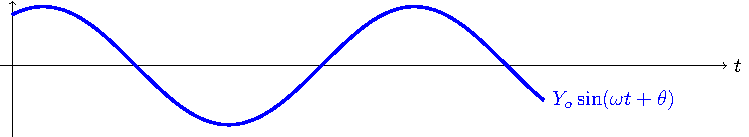
\includegraphics[width=.9\linewidth]{../figs/sin.pdf}
		\caption{Ejemplo de forma de onda sinusoidal}
		\label{fig.sin}
	\end{figure}
	
	La fase representa el argumento de la onda para $t=0$. Tomando una onda como referencia, si la fase de otra onda es $0^\circ$, se dice que la onda está \textbf{en fase} con la onda de referencia; si la fase es positiva ($+$) respecto a la de referencia, se dice que la onda está \textbf{en adelanto}; y si la fase es negativa ($-$) respecto a la de referencia, se dice que la onda está \textbf{en retraso}. Así, en la Figura~\ref{fig.desfase}, considerando como referencia la onda de color negro (que tiene una fase $\theta=0$), la {\color{blue} onda azul} está en retraso, mientras que la {\color{red} onda roja} está en adelanto. En caso de que el desfase entre dos ondas sea de 90$^\circ$, se dice que están \textbf{en cuadratura}: el paso por 0 de una onda, coincide con el paso por el máximo/mínimo de la otra.
	\begin{figure}[H]
		\centering
		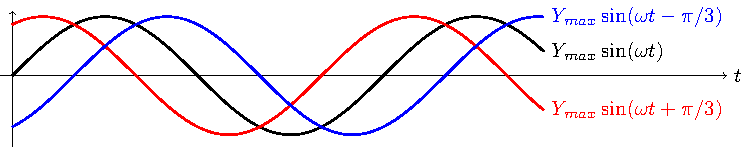
\includegraphics[width=.9\linewidth]{../figs/desfase.pdf}
		\caption{Fases entre ondas sinusoidales}
		\label{fig.desfase}
	\end{figure}
	
	
	Las propiedades de las formas de onda senoidales que hacen que sea la preferida para la generación de energía eléctrica a gran escala son las siguientes:
	\begin{enumerate}
		\item Su forma básica se mantiene siempre, puesto que sus derivadas e integrales sucesivas son funciones sinusoidales $\rightarrow$ si la excitación es sinusoidal, las respuestas también lo son (pasado un corto periodo de tiempo transitorio)
		\item La suma o resta de funciones senoidales de la misma frecuencia es otra función senoidal de la misma frecuencia
	\end{enumerate}
	Respecto al estudio de otras formas de onda, su interés reside en el teorema de Fourier, dado que cualquier onda periódica no senoidal puede suponerse formada por infinitas ondas senoidales de distinta frecuencia. 
	
	Al ser un caso particular de una onda periódica, las definiciones y valores de interés indicados previamente también son válidos. Por simplicidad, se considera la función sinusoidal con fase inicial nula, $y(t)=Y_{max}\cdot\sin(\omega t)$:
	\begin{itemize}
		\item \textbf{Valor pico a pico ($Y_{PP}$)}: es el doble de la amplitud: 
		\begin{equation*}
			Y_{PP}=|Y_{max} - Y_{min}|=2\cdot Y_{max}
		\end{equation*}
		\item \textbf{Valor medio ($Y_m$)}: en un periodo, el valor medio es 0, puesto que el área positiva es igual al área negativa. Considerando entonces un semiperíodo: 
		\begin{equation*}
			Y_m(T/2)=\frac{1}{T/2}\int_{0}^{T/2} Y_{max}\cdot \sin(\omega t)\, dt=\dfrac{2\cdot Y_{max}}{T\cdot\omega}\left[-\cos(\omega\cdot t)\right]_0^{T/2} =\dfrac{2\cdot Y_{max}}{\pi}\approx 0.637\cdot Y_{max}
		\end{equation*}
		\item \textbf{Valor eficaz ($Y_{ef}$)}: para simplificar el cálculo, se hace en primer lugar el valor eficaz al cuadrado:
		\begin{equation*}
			Y_{ef}^2=\dfrac{1}{T}\cdot\int_{0}^{T}\left(Y_{max}\cdot\sin(\omega  t)\right)^{2}\,dt=\dfrac{Y_{max}^2}{T}\cdot\int_{0}^{T}\left(\sin(\omega t)\right)^{2}\,dt=\dfrac{Y_{max}^2}{2}
		\end{equation*}
		luego:
		\begin{equation*}
			Y_{ef}=\sqrt{Y_{ef}^2}=\dfrac{Y_{max}}{\sqrt{2}}\approx0.707\cdot Y_{max}
		\end{equation*}
		\item \textbf{Factor de amplitud ($FA$)}: 
		\begin{equation*}
			FA = \dfrac{Y_{max}}{Y_{ef}}=\dfrac{\cancel{Y_{max}}}{\frac{\cancel{Y_{max}}}{\sqrt{2}}}=\sqrt{2}\approx 1.414
		\end{equation*}
		\item \textbf{Factor de forma ($FF$)}: 
		\begin{equation*}
			FF = \dfrac{Y_{ef}}{Y_{m}} = \dfrac{\frac{\cancel{Y_{max}}}{\sqrt{2}}}{\frac{2\cdot \cancel{Y_{max}}}{\pi}}=\dfrac{\pi}{2\cdot\sqrt{2}}\approx 1.111
		\end{equation*}
	\end{itemize}
	
	\subsection{Cálculo fasorial}
	
	Cuando se trabaje con corriente alterna, siempre se usarán funciones de onda sinusoidales, todas ellas de la misma pulsación $\omega$. Por tanto, las diferencias que habrá en dichas ondas serán, únicamente, las amplitudes $Y_{max}$ y las fases $\theta$. Esto permite que, en lugar de trabajar con formas de onda, se pueda trabajar con \textbf{fasores}, números complejos que representan una tensión o corriente sinusoidales. %Un fasor es un vector giratorio, anclado en el origen del plano complejo, que gira en el sentido contrario a las agujas del reloj a velocidad angular constante $\omega$. 
	La longitud del fasor (su módulo) es el \textbf{valor eficaz} de la función sinusoidal, que se define como el valor de la corriente alterna que consigue generar el mismo resultado de tensión/corriente que si fuera en corriente continua, y se calcula como el valor máximo entre $\sqrt{2}$ (como ya se justificó). 
% 	\begin{remark}
% 	    En realidad, el \textbf{módulo} del fasor puede ser el valor máximo, medio o eficaz de la onda, según interese. En general, y salvo que no se indique lo contrario, se considerará que el módulo del fasor es el \textbf{valor eficaz}.
% 	\end{remark}
	La posición del fasor, conocida como argumento, se determina en cualquier instante de tiempo haciendo el producto $\omega t+\theta$, pero la de más interés es el instante inicial, es decir, para $t=0$ en la expresión~\eqref{eq.y_senoidal}:
	\begin{equation*}
		y(t)=Y_{max}\cdot\sin(\cancelto{0}{\omega \cdot 0}+\theta)=Y_{max}\cdot\sin(\theta)
	\end{equation*}
	Por simplicidad, la fase $\theta$, al trabajar con fasores, puede expresarse en grados [$^\circ$]. Por tanto, al fasor le corresponde por módulo y argumento:
	\begin{equation}
		\boxed{\overline{Y}=Y_{ef}\,\phase{\theta}}
	\end{equation}
	que es conocida como la \textbf{forma polar} del fasor.
	
	\begin{example}
		\textbf{Expresar en modo de fasor las siguientes funciones sinusoidales:}
		\begin{align*}
		    u(t)&=150\,\sqrt{2}\cdot \sin(500\cdot t+\frac{\pi}{4})\, V\\
		    i(t) &= 3\,\sqrt{2}\cdot \sin(2000\cdot t+\frac{\pi}{6})\,A
		\end{align*}
		
		Para expresar los fasores, hay que utilizar los valores eficaces ($U_{ef}=150$ V; $I_{ef}=3$ A) y los desfases ($\frac{\pi}{4}=45^\circ$ para la $u(t)$ y $\frac{\pi}{6}=60^\circ$ para la $i(t)$). Así: 
		\begin{align*}
		    \overline{U}&=150\phase{45^\circ} V\\
		    \overline{I}&=3\phase{30^\circ}\,A
		\end{align*}
	\end{example}
	
%  	\section{Conceptos fundamentales}
% 	Como ya se mencionó en el Tema~\ref{chap.cc}, la corriente alterna monofásica se basa en ondas sinusoidales, que se expresan de forma matemática como:
% 	\begin{equation}\label{eq.y_senoidal}
% 		\boxed{y(t)=Y_{max}\cdot\sin(\omega t+\theta)} 
% 	\end{equation}
% 	siendo $Y_{max}$ el valor máximo de la onda, $\omega$ la pulsación o frecuencia angular [rad/s] ($\omega=2\cdot\pi\cdot f$, siendo $f$ la frecuencia de la onda [Hz]) y $\theta$ la fase/desfase [rad o $^\circ$]. 


% 	Se recuerda, además, que en el caso de las ondas sinusoidales, el valor medio en un periodo es 0 ($Y_m=0$), y el valor eficaz: 
% 	\begin{equation}
% 		\boxed{Y_{ef}=\dfrac{Y_{max}}{\sqrt{2}}\approx0.707\cdot Y_{max}}
% 	\end{equation}
	
% 	\section{Cálculo fasorial}
	Considerando la Figura~\ref{fig.fasor}, donde el \texttt{eje X} representa la parte real del fasor y, el \texttt{eje Y}, la parte imaginaria, la \textbf{forma binómica} (o rectangular) de un fasor, se obtiene como: 
	\begin{equation}
		\boxed{\overline{Y} = Y_{ef}\cdot(\cos(\theta)+\mathrm{j}\cdot\sin(\theta))}
	\end{equation}
	\begin{figure}[H]
		\centering
		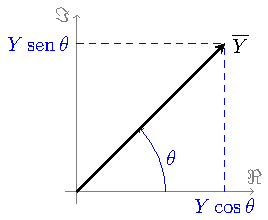
\includegraphics{../figs/fasor.pdf}
		\caption{Concepto de fasor}
		\label{fig.fasor}
	\end{figure}
	
	El empleo de estas notaciones permite operar con las funciones sinusoidales del mismo modo que con vectores en el plano y números complejos. En general, es habitual emplear la \textbf{forma binómica} para sumar y restar, y la \textbf{forma polar} para multiplicar y dividir. Debe tenerse en cuenta que para realizar estas operaciones es necesario que las expresiones sean todas con la función \texttt{seno} o con \texttt{coseno}. Caso contrario, habrá que expresar todas las magnitudes respecto a la misma función, siguiendo la relación: 
	\begin{equation*}
		\cos(\beta)=\sin(\beta+90^\circ)
	\end{equation*}
	\begin{remark}
		Si se tiene un fasor en forma rectangular $a+\mathrm{j}\,b$, para transformarlo a polar se debe calcular su módulo $\sqrt{a^2+b^2}$ y argumento $\arctan(b/a)$.
	\end{remark}
	
	\begin{remark}
		Si se tiene un fasor en forma polar $r\phase{\alpha^\circ}$, para transformarlo a rectangular se debe calcular $a$ como $r\cdot \cos(\alpha^\circ)$ y $b$ como $r\cdot \sin(\alpha^\circ)$.
	\end{remark}
	
	\begin{remark}
		Se recuerda que el empleo de fasores solo es válido cuando todas las ondas tienen la misma pulsación $\omega$
	\end{remark}
	
	\vspace{4mm}
	\begin{example}
		\textbf{Dados $\overline{U_1}=25\phase{145}^\circ$ V y $\overline{U_2}=11\phase{25^\circ}$ V, calcular la relación $\overline{U_1}/\overline{U_2}$ y la suma $\overline{U_1}+\overline{U_2}$.}
		
		Para hacer el cociente se utiliza la forma polar: 
		\begin{equation*}
			\dfrac{\overline{U_1}}{\overline{U_2}}=\dfrac{25\phase{145^\circ}}{11\phase{25^\circ}}=\dfrac{25}{11}\phase{145^\circ-25^\circ}=2.27\phase{120^\circ}
		\end{equation*}
		
		Para hacer la suma, es necesario usar la forma binómica:
		\begin{align*}
		    \overline{U_1}&=25\phase{145^\circ}=-20.48+\mathrm{j} 14.34 V\\
		    \overline{U_2}&=11\phase{30^\circ}=9.52+\mathrm{j} 5.5 V
		\end{align*}
		
		La suma de ambas tensiones es: 
		\begin{equation*}
			\overline{U_1}+\overline{U_2}=(-20.48+\mathrm{j}14.34)+(9.52+\mathrm{j}5.5)=-10.96+\mathrm{j}19.84
		\end{equation*}
	\end{example}
	
	\vspace{4mm}
	\begin{example}
		\textbf{Sabiendo que $i_1(t)=2\cdot\sqrt{2}\cdot \sin(600\cdot t)$ A; $i_2(t)=4\cdot\sqrt{2}\cdot \sin\left(600\cdot t+\frac{\pi}{2}\right)$ A; e $i_3(t)=10\cdot\sqrt{2}\cdot \cos(600\cdot t-\pi)$ A, determinar la suma de $i_1(t)+i_2(t)+i_3(t)$.}
		
		En primer lugar, se expresa todo en funciones seno: 
		\begin{align*}
			i_1(t)&=2\cdot\sqrt{2}\cdot \sin(600\cdot t)\rightarrow \overline{I_1}=2\phase{0^\circ}\;\text{A}\\
			i_2(t)&=4\cdot\sqrt{2}\cdot \sin\left(600\cdot t+\frac{\pi}{2}\right)\rightarrow \overline{I_2}=4\phase{90^\circ}\;\text{A}\\
			i_3(t)&=10\cdot\sqrt{2}\cdot \cos(600\cdot t-\pi)=10\cdot\sqrt{2}\cdot \sin\left(600\cdot t-\frac{\pi}{2}\right)\rightarrow \overline{I_3}=10\phase{-90^\circ}\;\text{A}\
		\end{align*}
		
		Así, la suma de $i_1(t)+i_2(t)+i_3(t)$ es:
		\begin{align*}
			\overline{I_1}&+\overline{I_2}+\overline{I_3}=(2\phase{0^\circ})+(4\phase{90^\circ})+(10\phase {-90^\circ})=6.32\phase{-71.5651^\circ}\;\text{A} \\
			&i_1(t)+i_2(t)+i_3(t)=6.32\cdot\sqrt{2}\cdot \sin(600\cdot t-1.249)\;\text{A}
		\end{align*}
	\end{example}
	
	\subsection{Representación fasorial: diagramas fasoriales}
	
	Considérense las ondas de tensión $u(t)$ y corriente $i(t)$ mostradas en la Figura~\ref{fig.ondasTensionCorriente}, representadas en notación fasorial como:
	\begin{equation*}
		\overline{U} = U\phase{\theta_U};\qquad\qquad   \overline{I} = I\phase{\theta_I}
	\end{equation*}
	donde $U$ e $I$ son los valores eficaces de la tensión y corriente, respectivamente. Su representación gráfica en el plano es la mostrada en la Figura~\ref{fig.fasortensioncorriente}. A estos diagramas se los conoce como \textbf{diagramas fasoriales}, y permiten también el estudio y análisis de circuitos en corriente alterna como si de vectores en el plano se tratara. Además, este procedimiento gráfico ofrece la ventaja, respecto al procedimiento algebraico, de que las relaciones de fase y amplitud entre todas las tensiones e intensidades quedan expuestas de forma muy clara e intuitiva. Por tanto, a lo largo de este Tema~\ref{chap.ca_mono} se irán realizando y analizando los diagramas fasoriales correspondientes a los circuitos en estudio.
	
	\begin{figure}[H]
		\centering
		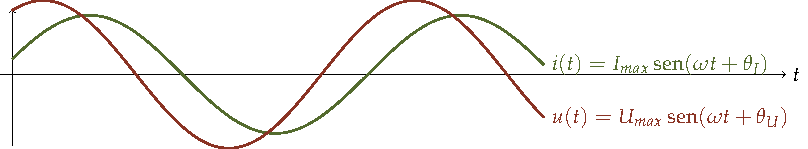
\includegraphics[width=.9\linewidth]{../figs/ondasTensionCorriente.pdf}
		\caption{Tensión y corriente en notación fasorial}
		\label{fig.ondasTensionCorriente}
	\end{figure}
	
	
	\begin{figure}[H]
		\centering
		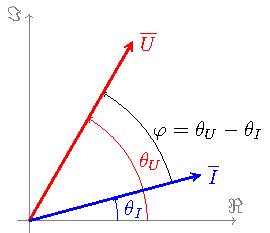
\includegraphics[width=0.3\linewidth]{../figs/fasorTensionCorriente.pdf}
		\caption{Diagrama fasorial de $\overline{U}$ e  $\overline{I}$}
		\label{fig.fasortensioncorriente}
	\end{figure}
	
	\begin{remark}
		A partir de este momento, se utilizará siempre $U$ para referirse a tensión eficaz e $I$ para la corriente eficaz.
	\end{remark}
	
	\section{Respuesta de los elementos pasivos a una excitación sinusoidal}
	
	La ley de Ohm también puede escribirse utilizando fasores, de manera que: 
	\begin{equation}\label{eq.ohm_generalizada}
		\boxed{ \overline{U}=\overline{Z}\cdot\overline{I} }
	\end{equation}
	siendo la impedancia:
	\begin{equation}\label{eq.impedancia}
		\boxed{\overline{Z} = \frac{U}{I}\phase{\theta_U - \theta_I} \Rightarrow 
			\begin{cases}
				Z = \frac{U}{I}\\
				\theta = \theta_U - \theta_I
		\end{cases}}
	\end{equation}
	Por tanto, la impedancia $\overline{Z}=Z\phase{\theta}$ es el cociente entre tensión y corriente [$\Omega$]. De nuevo, la expresión para la impedancia mostrada en la ecuación~\eqref{eq.impedancia} se presenta en forma polar, siendo en forma binómica: 
	\begin{equation*}
		\overline{Z} = Z\cdot\cos(\theta)+\mathrm{j}\,Z\cdot\sin(\theta) %= R + \mathrm{j} X
	\end{equation*}
	cuyo resultado, según se demostrará más adelante, es igual a: 
	\begin{equation}
		\boxed{\overline{Z} =  R + \mathrm{j} X}
	\end{equation}
	donde $R$ es la parte resistiva de la impedancia (resistencia), y $X$ es la parte reactiva (bobina y/o condensador), como se muestra en la Figura~\ref{fig.fasorimpedancia}. La parte imaginaria de $\overline{Z}$ (la $X$) puede ser positiva (reactancia inductiva $\rightarrow$ bobina) o negativa (reactancia capacitiva $\rightarrow$ condensador). Además, una impedancia puede ser puramente resistiva ($Z=R$), inductiva ($Z=+X$) o capacitiva ($Z=-X$).
	\begin{figure}[H]
		\centering
		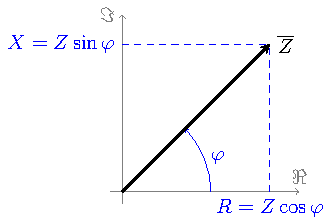
\includegraphics{../figs/fasorImpedancia.pdf}
		\caption{Fasor de una impedancia genérica $\overline{Z}$}
		\label{fig.fasorimpedancia}
	\end{figure}
	
	\begin{remark}
		Cuando los elementos pasivos son puramente reactivos, la impedancia se conoce como reactancia $X$ y, la admitancia, como susceptancia $B$.
	\end{remark}
	
	% A modo de resumen, la Tabla \ref{tab.relaciones_rlc2} muestra las relaciones entre tensión y corriente en los diferentes elementos pasivos simples. En las Secciones~\ref{sec.R-puro}--\ref{sec.C-puro} se justifican dichas relaciones.
	% \begin{table}[H]
		%     \centering
		%     \begin{tabular}{c|c|c}
			%         \rowcolor{ocre!50} \textbf{Elemento} & \textbf{$i(t)=I\sqrt{2}\cdot \sin(\omega t)$} & \textbf{$u(t)=U\sqrt{2}\cdot \sin(\omega\cdot t)$} \\[3pt]
			%         R & $u_R=R\cdot I\sqrt{2}\cdot \sin(\omega t)$ & $i_R=\dfrac{U\sqrt{2}}{R}\cdot \sin(\omega t)$\\ [10pt]
			%         L & $u_L=\omega\cdot L\cdot I\sqrt{2}\cdot \sin(\omega t+\frac{\pi}{2})$ & $i_L =\dfrac{U\sqrt{2}}{\omega\cdot L}\cdot \sin(\omegat)$ \\ [10pt]
			%         C & $u_C=\dfrac{I_m}{\omega\cdot C}\cdot cos(\omega\cdot t)$ & $i_C =\omega\cdot C\cdot V_m\cdot cos(\omega\cdot t+90)$\\
			%     \end{tabular}
		%     \caption{Relaciones de los elementos pasivos: corriente alterna sinusoidal}
		%     \label{tab.relaciones_rlc2}
		% \end{table}
		
		\subsection{Circuito resistivo}\label{sec.R-puro}
	
	Considérese una resistencia $R$ por la que circula una corriente alterna de forma de onda:
	\begin{equation*}
		i(t)=I\,\sqrt{2}\cdot\sin(\omega t+\theta_I)\rightarrow\overline{I}=I\phase{\theta_I}
	\end{equation*}
	Aplicando la ley de Ohm, la tensión en los bornes de la resistencia es:
	\begin{equation*}
		u(t)=R\cdot i(t) ={\color{blue}R\cdot I}\,\sqrt{2}\cdot\sin(\omega t+{\color{red}\theta_I})={\color{blue}U}\,\sqrt{2}\cdot\sin(\omega t+{\color{red}\theta_U})\,,
	\end{equation*}
	función senoidal que va \textbf{en fase} con la intensidad (Figura~\ref{fig.resistivo}), y cuyo valor eficaz es $U=R\cdot I$. Por tanto, le corresponde el fasor
	\begin{equation*}
		\overline{U}=(R\cdot I)\phase{0+\theta_I}=U\phase{\theta_U}
	\end{equation*}
	donde $\theta_I=\theta_U$.
	\begin{figure}[H]
		\centering
		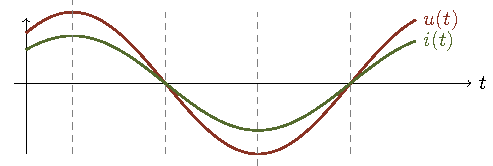
\includegraphics{../figs/resistivo.pdf}
		\caption{$u(t)$ e $i(t)$ en circuitos resistivos puros}
		\label{fig.resistivo}
	\end{figure}
	
	Así, la impedancia $\overline{Z_R}$, según la expresión~\eqref{eq.impedancia}:
	\begin{equation*}
		\overline{Z_R}=\dfrac{\overline{U}}{\overline{I}}\Rightarrow
		\begin{cases}
			Z_R=\dfrac{U}{I}=R\\
			\theta=\theta_U-\theta_I=0
		\end{cases}
	\end{equation*}
	Es decir, que la impedancia de una resistencia tiene de módulo el valor de la resistencia y un argumento nulo: 
	\begin{equation}\label{eq.resistencia}
		\boxed{ \overline{Z_R}=R+\mathrm{j}\,0=R\phase{0^\circ}}
	\end{equation}
	La representación fasorial de $\overline{U}$ e $\overline{I}$, así como la de $\overline{Z_R}$, se muestran en la Figura~\ref{fig.fasorResistencia}. 
	\begin{figure}[H]
		\centering
		\subfloat[$\overline{U}$ e $\overline{I}$]{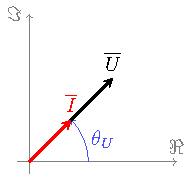
\includegraphics[width=0.2\linewidth]{../figs/fasorResistencia_VI.pdf}}\hfil
		\subfloat[$\overline{Z_R}$]{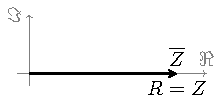
\includegraphics[width=0.22\linewidth]{../figs/fasorResistencia.pdf}}
		\caption{Diagrama fasorial de un circuito resistivo puro}
		\label{fig.fasorResistencia}
	\end{figure}
	
	\subsection{Circuito inductivo puro}\label{sec.L-puro}
	
	Considérese una bobina de inductancia $L$ por la que circula una corriente alterna de forma de onda:
	\begin{equation*}
		i(t)=I\,\sqrt{2}\cdot\sin(\omega t+\theta_I)\rightarrow\overline{I}=I\phase{\theta_I}
	\end{equation*}
	Según se indica en la expresión~\eqref{eq.u_L}, la relación entre tensión y corriente en una bobina es: 
	\begin{equation*}
		u(t)=L\cdot\dfrac{di(t)}{dt}={\color{blue}L\cdot I \cdot \omega}\,\sqrt{2}\cdot  \cos(\omega t+{\color{red}\theta_I})= {\color{blue} U} \sqrt{2}\cdot \omega\cdot  \sin \left(\omega t+{\color{red}\theta_I+\frac{\pi}{2}}\right)= {\color{blue} U} \sqrt{2}\cdot \omega\cdot  \sin \left(\omega t+{\color{red}\theta_U}\right)\,
	\end{equation*}
	Así, un circuito inductivo puro genera señales en cuadratura entre $u(t)$ e $i(t)$, estando la corriente \textbf{retrasada 90$^\circ$} respecto a la tensión (Figura~\ref{fig.inductivoPuro}). A la tensión le corresponde el fasor:
	\begin{equation*}
		\overline{U}=(L\cdot I\cdot\omega)\phase{\theta_I+\frac{\pi}{2}}=U\phase{\theta_U}
	\end{equation*}
	\begin{figure}[H]
		\centering
		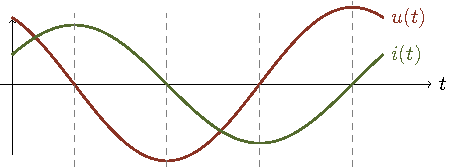
\includegraphics{../figs/inductivoPuro.pdf}
		\caption{$u(t)$ e $i(t)$ en circuitos inductivos puros}
		\label{fig.inductivoPuro}
	\end{figure}
	
	Por tanto, la impedancia $\overline{Z_L}$, según la expresión~\eqref{eq.impedancia}:
	\begin{equation*}
		\overline{Z_L}=\dfrac{\overline{U}}{\overline{I}}\Rightarrow
		\begin{cases}
			Z_L=\dfrac{U}{I}=\omega\cdot L\\
			\theta=\theta_U-\theta_I=90^\circ
		\end{cases}
	\end{equation*}
	Es decir, que la impedancia de una bobina tiene de módulo el valor $L\cdot\omega$, conocido como \textbf{reactancia inductiva} (resistencia aparente que ofrece la bobina al paso de la corriente alterna) y un argumento de $+90^\circ$:
	\begin{equation}
		\boxed{0+\mathrm{j}\,L\omega=L\omega\phase{90^\circ}}
	\end{equation}
	La representación fasorial de $\overline{U}$ e $\overline{I}$, así como la de $\overline{Z_L}$, se muestran en la Figura~\ref{fig.fasorInductancia}. 
	\begin{figure}[H]
		\centering
		\subfloat[$\overline{U}$ e $\overline{I}$]{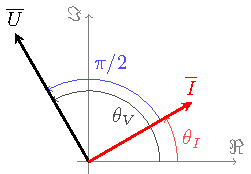
\includegraphics[width=0.28\linewidth]{../figs/fasorInductancia_VI.pdf}}\hfil
		\subfloat[$\overline{Z_L}$]{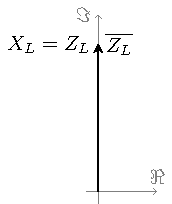
\includegraphics[width=0.19\linewidth]{../figs/fasorInductancia.pdf}}
		\caption{Diagrama fasorial de un circuito inductivo puro}
		\label{fig.fasorInductancia}
	\end{figure}
	
	\subsection{Circuito capacitivo puro}\label{sec.C-puro}
	
	Considérese un condensador de capacidad $C$ por el que circula una corriente alterna de forma de onda:
	\begin{equation*}
		i(t)=I\,\sqrt{2}\cdot\sin(\omega t+\theta_I)\rightarrow\overline{I}=I\phase{\theta_I}
	\end{equation*}
	Según se indica en la expresión~\eqref{eq.u_C}, la relación entre tensión y corriente en un condensador, (considerando que $t_i=-\infty$ y que $u(-\infty)=0$) es: 
	\begin{equation*}
		u(t)=\dfrac{1}{C}\cdot\int_{-\infty}^{t} i(t)\cdot dt=-{\color{blue}\dfrac{I}{\omega\,C}}\sqrt{2}\cdot\cos (\omega t+{\color{red}\theta_I})={\color{blue}U}\sqrt{2}\cdot\sin \left(\omega t+{\color{red}\theta_I-\frac{\pi}{2}}\right)
	\end{equation*}
	Así, un circuito capacitivo puro genera señales en cuadratura entre $u(t)$ e $i(t)$, estando la corriente \textbf{adelantada 90$^\circ$} respecto a la tensión (Figura~\ref{fig.capacitivoPuro}). A la tensión le corresponde el fasor:
	\begin{equation*}
		\overline{U}=\left( \dfrac{I}{\omega C} \right)\phase{\theta_I-\frac{\pi}{2}}=U\phase{\theta_U}
	\end{equation*}
	\begin{figure}[H]
		\centering
		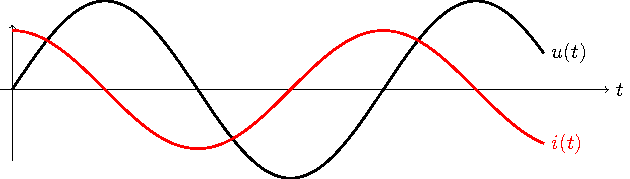
\includegraphics{../figs/capacitivoPuro.pdf}
		\caption{$u(t)$ e $i(t)$ en circuitos capacitivos puros}
		\label{fig.capacitivoPuro}
	\end{figure}
	
	Por tanto, la impedancia $\overline{Z_C}$, según la expresión~\eqref{eq.impedancia}:
	\begin{equation*}
		\overline{Z_C}=\dfrac{\overline{U}}{\overline{I}}\Rightarrow
		\begin{cases}
			Z_C=\dfrac{U}{I}=\dfrac{1}{\omega C}\\
			\theta=\theta_U-\theta_I=-90^\circ
		\end{cases}
	\end{equation*}
	Es decir, que la impedancia de un condensador tiene de módulo el valor $\frac{1}{\omega C}$, conocido como \textbf{reactancia capacitiva} (resistencia aparente que ofrece el condensador al paso de la corriente alterna) y un argumento de $-90^\circ$:
	\begin{equation}
		\boxed{0-\mathrm{j}\,\dfrac{1}{\omega C}=\dfrac{1}{\omega C}\phase{-90^\circ}}
	\end{equation}
	La representación fasorial de $\overline{U}$ e $\overline{I}$, así como la de $\overline{Z_C}$, se muestran en la Figura~\ref{fig.fasorCondensador}. 
	\begin{figure}[H]
		\centering
		\subfloat[$\overline{U}$ e $\overline{I}$]{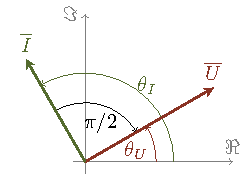
\includegraphics[width=0.28\linewidth]{../figs/fasorCondensador_VI.pdf}}\hfil
		\subfloat[$\overline{Z_C}$]{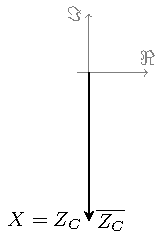
\includegraphics[width=0.19\linewidth]{../figs/fasorCondensador.pdf}}
		\caption{Diagrama fasorial de un circuito capacitivo puro}
		\label{fig.fasorCondensador}
	\end{figure}
	
	\section{Respuesta de los circuitos serie a una excitación senoidal} \label{sec.respuesta_serie}
	
	\subsection{Circuito $RL$}\label{sec.RL}
	
	Este circuito se corresponde con el mostrado en la Figura~\ref{fig.RL}, equivalente a un circuito inductivo con pérdidas. 
	\begin{figure}[H]
		\centering
		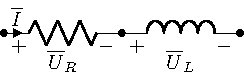
\includegraphics[width=0.3\linewidth]{../figs/RL.pdf}
		\caption{Circuito $RL$ serie}
		\label{fig.RL}
	\end{figure}
	
	La corriente que circula por el circuito es:
	\begin{equation*}
		i(t)=I\,\sqrt{2}\cdot\sin(\omega t+\theta_I)\rightarrow\overline{I}=I\phase{\theta_I}
	\end{equation*}
	por lo que las tensiones en la resistencia $R$ y bobina $L$:
	\begin{align*}
		u_R(t)=R\, I\,\sqrt{2}\cdot\sin(\omega t+\theta_I)&\rightarrow \overline{U_R} = R \overline{I}=R\,I\phase{\theta_I}\\ 
		u_L(t)= \omega\,L\,I \sqrt{2}\cdot \sin \left(\omega t+\theta_I+\frac{\pi}{2}\right)&\rightarrow \overline{U_L}=\overline{X_L}\cdot\overline{I}= \omega\,L\,I\phase{\theta_I+90^\circ}
	\end{align*}
	donde $u_R(t)$ va en fase con $i(t)$ y $u_L(t)$ va 90$^\circ$ adelantada respecto a $i(t)$.  
	
	La impedancia del circuito (resistencia aparente que ofrece al paso de la corriente alterna) es el conjunto de $R$ y $L$, que se corresponde con una magnitud compleja: 
	\begin{equation}
		\boxed{ \overline{Z} = R + \mathrm{j}\,X_L = R+ \mathrm{j}\,\omega L \Rightarrow 
			\begin{cases}
				Z=\sqrt{R^2+(\omega L)^2}\\
				\theta=\arctan\left(\dfrac{\omega\,L}{R} \right)
		\end{cases}}
	\end{equation}
	que puede representarse en el plano complejo como se muestra en la Figura~\ref{fig.fasorinductanciareal}, donde es inmediato comprobar que:
	\begin{align*}
		R&=Z\cdot\cos(\theta)\\
		X_L&=Z\cdot\sin(\theta)
	\end{align*} 
	\begin{figure}[H]
		\centering
		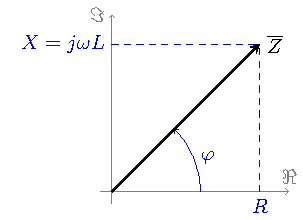
\includegraphics{../figs/fasorInductanciaReal.pdf}
		\caption{Representación gráfica de la impedancia de un circuito $RL$}
		\label{fig.fasorinductanciareal}
	\end{figure}
	
	
	La tensión total del circuito, según la 2LK, es:  
	\begin{equation*}
		\overline{U} = \overline{U_R} + \overline{U_L} =(R + \mathrm{j}\,\omega L) \cdot \overline{I}\Rightarrow 
		\begin{cases}
			U=\sqrt{U_R^2+U_L^2}=I\sqrt{R^2+(\omega L)^2}=I\cdot Z\\
			\theta=\arctan\left( \dfrac{U_L}{U_R}\right)=\arctan\left( \dfrac{\omega L}{R}\right)
		\end{cases}
	\end{equation*}
	Por tanto, la intensidad $i(t)$ va \textbf{retrasada} respecto a la tensión total $u(t)$, pero \textbf{no en cuadratura} con ésta  (Figura~\ref{fig.fasorInductanciaReal_VI}).
	
	\begin{figure}[H]
		\centering
		\subfloat[Evolución temporal]{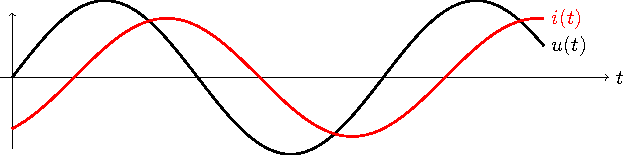
\includegraphics[width=0.7\linewidth]{../figs/inductivo.pdf}}\hfil
		\subfloat[Diagrama fasorial]{    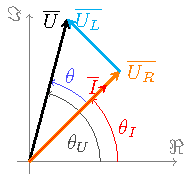
\includegraphics{../figs/fasorInductanciaReal_VI.pdf}}
		\caption{Evolución temporal y diagrama fasorial de $u(t)$ e $i(t)$ en circuitos $RL$}
		\label{fig.fasorInductanciaReal_VI}
	\end{figure}
	
	
	
	\subsection{Circuito $RC$}\label{sec.RC}
	
	Este circuito se corresponde con el mostrado en la Figura~\ref{fig.RC}, equivalente a un circuito capacitivo con pérdidas. 
	\begin{figure}[H]
		\centering
		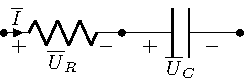
\includegraphics{../figs/RC.pdf}
		\caption{Circuito $RC$ serie}
		\label{fig.RC}
	\end{figure}
	
	La corriente que circula por el circuito es:
	\begin{equation*}
		i(t)=I\,\sqrt{2}\cdot\sin(\omega t+\theta_I)\rightarrow\overline{I}=I\phase{\theta_I}
	\end{equation*}
	por lo que las tensiones en la resistencia $R$ y el condensador $C$:
	\begin{align*}
		u_R(t)=R\, I\,\sqrt{2}\cdot\sin(\omega t+\theta_I)&\rightarrow \overline{U_R} = R \overline{I}=R\,I\phase{\theta_I}\\ 
		u_C(t)=\dfrac{I\,\sqrt{2}}{\omega\,C} \cdot \sin \left(\omega t+\theta_I-\frac{\pi}{2}\right)&\rightarrow \overline{U_C}=\overline{X_C}\cdot\overline{I}=\dfrac{I}{\omega C}\phase{\theta_I-90^\circ}
	\end{align*}
	donde $u_R(t)$ va en fase con $i(t)$ y $u_C(t)$ va 90$^\circ$ retrasada respecto a $i(t)$. 
	
	La impedancia del circuito (resistencia aparente que ofrece al paso de la corriente alterna) es el conjunto de $R$ y $C$, que se corresponde con una magnitud compleja: 
	\begin{equation}
		\boxed{ \overline{Z} = R + \mathrm{j}\,X_C = R- \mathrm{j}\dfrac{1}{\omega C} \Rightarrow 
			\begin{cases}
				Z=\sqrt{R^2-\left(\dfrac{1}{\omega C} \right)^2}\\
				\theta=-\arctan\left(\dfrac{\frac{1}{\omega\,C}}{R} \right)
		\end{cases}}
	\end{equation}
	que puede representarse en el plano complejo como se muestra en la Figura~\ref{fig.fasorcondensadorreal}, donde es inmediato comprobar que:
	\begin{align*}
		R&=Z\cdot\cos(\theta)\\
		X_C&=Z\cdot\sin(\theta)
	\end{align*} 
	\begin{figure}[H]
		\centering
		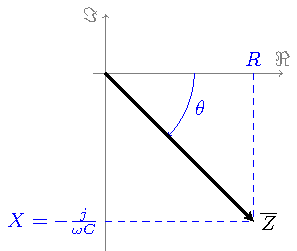
\includegraphics{../figs/fasorCondensadorReal.pdf}
		\caption{Representación gráfica de la impedancia de un circuito $RC$}
		\label{fig.fasorcondensadorreal}
	\end{figure}
	
	La tensión total del circuito, según la 2LK, es: 
	\begin{equation*}
		\overline{U} = \overline{U_R} + \overline{U_C} =\left(R - \mathrm{j}\,\dfrac{1}{\omega\,C}\right) \cdot \overline{I}\Rightarrow 
		\begin{cases}
			U=\sqrt{U_R^2+U_C^2}=I\sqrt{R^2+\left(\dfrac{1}{\omega\,C}\right)^2}=I\cdot Z\\
			\theta=-\arctan\left( \dfrac{U_C}{U_R}\right)=-\arctan\left( \dfrac{1}{R\,\omega\,C}\right)
		\end{cases}
	\end{equation*}
	Por tanto, la intensidad $i(t)$ va \textbf{adelantada} respecto a la tensión total $u(t)$, pero \textbf{no en cuadratura} con ésta  (Figura~\ref{fig.fasorCapacitivoReal_VI}). 
	\begin{figure}[H]
		\centering
		\subfloat[Evolución temporal]{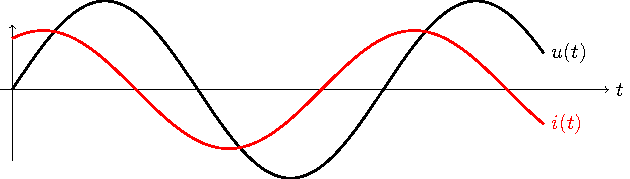
\includegraphics[width=0.7\linewidth]{../figs/capacitivo.pdf}}\hfil
		\subfloat[Diagrama fasorial]{    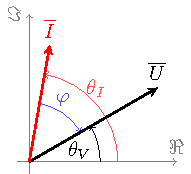
\includegraphics[width=0.28\linewidth]{../figs/fasorCondensadorReal_VI.pdf}}
		\caption{Evolución temporal y diagrama fasorial de $u(t)$ e $i(t)$ en circuitos $RC$}
		\label{fig.fasorCapacitivoReal_VI}
	\end{figure}
	
	\begin{remark}
		Se quiere destacar que, pese a que a una impedancia se le puede asociar un número complejo, no se trata de \textbf{un fasor} (señal que varía en el tiempo).
	\end{remark}
	
	\subsection{Circuito $RLC$}\label{sec.RLC}
	
	Este circuito se corresponde con el mostrado en la Figura~\ref{fig.RLC}. 
	\begin{figure}[H]
		\centering
		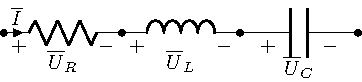
\includegraphics[width=0.4\linewidth]{../figs/RLC.pdf}
		\caption{Circuito $RLC$ serie}
		\label{fig.RLC}
	\end{figure}
	
	La corriente que circula por el circuito es:
	\begin{equation*}
		i(t)=I\,\sqrt{2}\cdot\sin(\omega t+\theta_I)\rightarrow\overline{I}=I\phase{\theta_I}
	\end{equation*}
	por lo que las tensiones en resistencia $R$, bobina $L$ y condensador $C$:
	\begin{align*}
		u_R(t)=R\, I\,\sqrt{2}\cdot\sin(\omega t+\theta_I)&\rightarrow \overline{U_R} = R \overline{I}=R\,I\phase{\theta_I}\\ 
		u_L(t)= \omega\,L\,I \sqrt{2}\cdot \sin \left(\omega t+\theta_I+\frac{\pi}{2}\right)&\rightarrow \overline{U_L}=\overline{X_L}\cdot\overline{I}= \omega\,L\,I\phase{\theta_I+90^\circ}\\
		u_C(t)=\dfrac{I\,\sqrt{2}}{\omega\,C} \cdot \sin \left(\omega t+\theta_I-\frac{\pi}{2}\right)&\rightarrow \overline{U_C}=\overline{X_C}\cdot\overline{I}=\dfrac{I}{\omega C}\phase{\theta_I-90^\circ}
	\end{align*}
	donde $u_R(t)$ va en fase con $i(t)$, $u_L(t)$ va 90$^\circ$ adelantada respecto a $i(t)$ y $u_C(t)$ va 90$^\circ$ retrasada respecto a $i(t)$. 
	
	La impedancia del circuito (resistencia aparente que ofrece al paso de la corriente alterna) es el conjunto de $R$, $L$ y $C$, que se corresponde con una magnitud compleja: 
	\begin{equation}
		\boxed{ \overline{Z} = R + \mathrm{j}\,(X_L-X_C) = R+ \mathrm{j}\left(\omega\,L-\dfrac{1}{\omega C}\right) \Rightarrow 
			\begin{cases}
				Z=\sqrt{R^2+\left(\omega L -\frac{1}{\omega C} \right)^2}\\
				\theta=\arctan\left(\dfrac{\omega L-\frac{1}{\omega\,C}}{R} \right)
		\end{cases}}
	\end{equation}
	que puede representarse en el plano complejo como se muestra en la Figura~\ref{fig.fasorRLC}, donde es inmediato comprobar que:
	\begin{align*}
		R&=Z\cdot\cos(\theta)\\
		X&=Z\cdot\sin(\theta)
	\end{align*} 
	\begin{figure}[H]
		\centering
		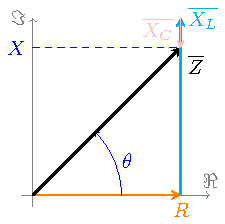
\includegraphics{../figs/fasorRLC.pdf}
		\caption{Representación gráfica de la impedancia de un circuito $RLC$}
		\label{fig.fasorRLC}
	\end{figure}
	
	La tensión total del circuito, según la 2LK, es: 
	\begin{equation*}
		\overline{U} = \overline{U_R} +\overline{U_L} + \overline{U_C} =\left(R+\mathrm{j}\,\omega\,L - \mathrm{j}\,\dfrac{1}{\omega\,C}\right) \cdot \overline{I}\Rightarrow 
		\begin{cases}
			U=I\sqrt{R^2 + \left(\omega L - \dfrac{1}{\omega C}\right)^2}=I\cdot Z\\
			\theta=\arctan\left( \dfrac{\omega\,L-\frac{1}{\omega\,C}}{R}\right)
		\end{cases}
	\end{equation*}
	Por tanto, \textit{a priori}, no se puede saber si la intensidad $i(t)$ va {adelantada o retrasada} respecto a la tensión total $u(t)$, puesto que dependerá de si $\overline{U_L}>\overline{U_C}\Rightarrow \omega L>\frac{1}{\omega C}$ (\textbf{carácter inductivo}) o $\overline{U_L}<\overline{U_C}\Rightarrow \omega L<\frac{1}{\omega C}$ (\textbf{carácter capacitivo}); además, también puede darse el caso de que $\overline{U_L}=\overline{U_C}\Rightarrow \omega L=\frac{1}{\omega C}$ (\textbf{carácter resistivo}), diciendo entonces que el circuito se encuentra \textbf{en resonancia} (ver Sección~\ref{sec.resonancia_serie}). En la Figura~\ref{fig.fasorRLC_VI} ha supuesto que la corriente va en retraso respecto a la tensión.
	\begin{figure}[H]
		\centering 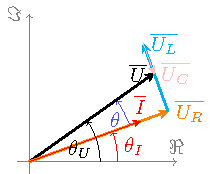
\includegraphics[width=0.3\linewidth]{../figs/fasorRLC_VI.pdf}
		\caption{Diagrama fasorial de un circuito $RLC$, suponiendo carácter inductivo}
		\label{fig.fasorRLC_VI}
	\end{figure}
	
	
	
	\subsection{Circuito serie general}
	Considérese un circuito en serie formado por $n$ impedancias, donde cada impedancia es de la forma $\overline{Z_i}=R_i+\mathrm{j}\,X_i$, como se muestra en la Figura~\ref{fig.serie-general-inicio}. Este circuito se alimenta con una tensión $u(t)$, de valor eficaz $U$, de manera que circula por el mismo una intensidad $i(t)$ de valor eficaz $I$. Se dice que la impedancia equivalente a las $n$ impedancias en serie es aquella que, al aplicarle la misma tensión $u(t)$, origina la misma intensidad $i(t)$, es decir, la que \textbf{conserva el módulo de $\overline{I}$ y el ángulo de fase} entre $\overline{U}$ e $\overline{I}$ del circuito serie original
	\begin{figure}[H]
		\centering
		\subfloat[Real]{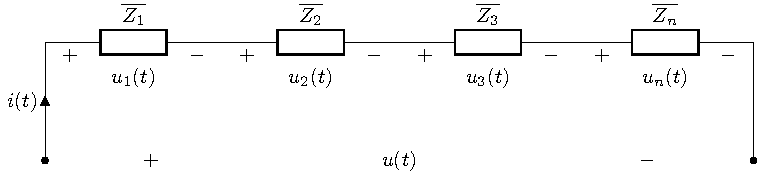
\includegraphics[height=2cm]{../figs/serie_general.pdf}\label{fig.serie-general-inicio}}\hfil
		\subfloat[Equivalente]{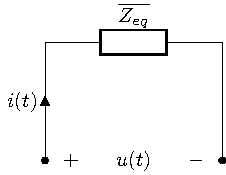
\includegraphics[height=2cm]{../figs/serie_general_eq.pdf}\label{fig.serie-general-eq}}
		\caption{Circuito serie general alimentado por corriente alterna}
		\label{fig.serie-general}
	\end{figure}
	
	En el acoplamiento de la Figura~\ref{fig.serie-general-inicio} se cumple que:
	\begin{equation*}
		\overline{U}=\overline{U_1}+\overline{U_2}+\overline{U_3}+...+\overline{U_n}
	\end{equation*}
	donde cada tensión es igual a $\overline{U_i}=\overline{I}\cdot\overline{Z_i}$, luego: 
	\begin{equation*}
		\overline{U}=\overline{U_1}+\overline{U_2}+\overline{U_3}+...+\overline{U_n}=\overline{I} \cdot(\overline{Z_1}+\overline{Z_2}+\overline{Z_3}+...+\overline{Z_n})
	\end{equation*}
	Puesto que en el circuito equivalente se cumple que: 
	\begin{equation*}
		\overline{U}=\overline{I}\cdot\overline{Z_{eq}}
	\end{equation*}
	se llega a la conclusión de que:
	\begin{equation}
		\overline{Z_{eq}}=\overline{Z_1}+\overline{Z_2}+\overline{Z_3}+...+\overline{Z_n}\Rightarrow \boxed{\overline{Z_{eq}}=\sum_{i=1}^n \overline{Z_i}}
	\end{equation}
	que equivale a decir que: 
	\begin{equation*}
		R_{eq}=\sum_{i=1}^n R_i\,;\qquad \qquad X_{eq}=\sum_{i=1}^n X_i
	\end{equation*}
	siendo el ángulo de la impedancia equivalente:
	\begin{equation*}
		\theta=\arctan\left(\dfrac{X_{eq}}{R_{eq}}\right)
	\end{equation*}
	
	\vspace{4mm}
	\begin{example}\label{ej.2-3}
		\textbf{Un circuito serie formado por $R=\qty{10}{\ohm}$, $L=\qty{20}{\milli\henry}$ y $C=\qty{100}{\micro\farad}$ es alimentado con una tensión $u(t)=200\cdot\sin(1000t+\frac{\pi}{4})\,\si{\volt}$. Calcular $\overline{I}$, ${u_R(t)}$, $u_L(t)$ y $u_C(t)$, y dibujar el diagrama fasorial de tensiones y corrientes.}

  \vspace{4mm}
		El valor eficaz de la tensión y su fase inicial son:
		\begin{equation*}
			U = \dfrac{U_{max}}{\sqrt{2}} =\dfrac{200}{\sqrt{2}} = 100\sqrt2\,\si{\volt} \;;\;\;\;\theta_U=\dfrac{\pi}{4}=45^\circ \quad \Rightarrow \quad\overline{U}=100\sqrt2\phase{\ang{45}}
		\end{equation*}
		Los valores de las impedancias $X_L$, $X_C$ y la impedancia equivalente son:
		\begin{align*}
			\overline{X}_L&=\mathrm{j}\,\omega\,L=\mathrm{j}\,1000\cdot20\cdot 10^{-3}= \mathrm{j}\,\qty{20}{\ohm}=20\phase{\ang{90}}\,\si{\ohm}\\
			\overline{X}_C&=-\mathrm{j}\,\dfrac{1}{\omega\,C}=\dfrac{1}{1000\cdot100\cdot 10^{-6}}= -\mathrm{j}\,\qty{10}{\ohm}=10\phase{\ang{-90}}\,\si{\ohm}		\\
			\overline{Z}_{eq}&=R+\overline{X}_L+\overline{X}_C=10+\mathrm{j}\,20-\mathrm{j}\,10=10+\mathrm{j}\,10\,\si{\ohm}=10\sqrt2 \phase{\ang{45}}\,\si{\ohm}
		\end{align*}
		Aplicando la ley de Ohm, se obtiene la corriente y, con ella, las tensiones de cada elemento:
		\begin{align*}
			\overline{I}&=\dfrac{\overline{U}}{\overline{Z}_{eq}}=\dfrac{100\sqrt2\phase{45^\circ}}{10\sqrt2\phase{45^\circ}}=10\phase{0^\circ}\,\si{\ampere}\\
			\overline{U}_R&=\overline{I}\cdot R=10\phase{0^\circ}\cdot 10=100\phase{0^\circ}\,\si{\volt} \quad \Rightarrow \quad u_R(t)=100\sqrt{2}\cdot\sin(1000t)\,\si{\volt}\\
			\overline{U}_L&=\overline{I}\cdot \overline{X}_L=10\phase{0^\circ}\cdot 20\phase{90^\circ}=200\phase{90^\circ}\,\si{\volt} \quad \Rightarrow \quad u_L(t)=200\sqrt{2}\cdot\sin\left(1000t+\tfrac{\pi}{2}\right)\,\si{\volt}\\
			\overline{U}_C&=\overline{I}\cdot \overline{X}_L=10\phase{0^\circ}\cdot 10\phase{-90^\circ} =100\phase{-90^\circ}\,\si{\volt} \quad \Rightarrow \quad u_C(t)=100\sqrt{2}\cdot\sin\left(1000t-\tfrac{\pi}{2}\right)\,\si{\volt}
		\end{align*}
		\begin{figure}[H]
			\centering
			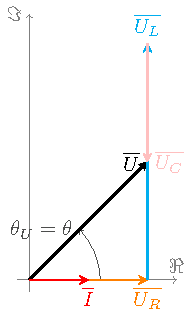
\includegraphics[]{../figs/diagrama_fasorial_ejemplo2_3.pdf}
			\caption{Diagrama fasorial del Ejemplo~\ref{ej.2-3}}
			\label{fig.diagrama_fasorial_ejemplo2-3}
		\end{figure}
		
	\end{example}
	
	\subsection{Resonancia}\label{sec.resonancia_serie}
	
	En un circuito serie $RLC$ se dice que se produce \textbf{resonancia} cuando la reactancia es nula:
	\begin{equation*}
		X=\omega\,L-\dfrac{1}{\omega\,C}=0\rightarrow \omega\,L=\dfrac{1}{\omega\,C}
	\end{equation*}
	Por tanto, cuando se produce resonancia, se tiene que $\overline{Z}=R$, siendo un circuito resistivo puro y $Z$ alcanzando su mínimo valor. Como, por ley de Ohm, $\overline{I}=\overline{U}/\overline{Z}$, la intensidad alcanzará su máximo valor y estará en fase con la tensión. 
	
	Para alcanzar resonancia, se puede llegar variando la autoinducción $L$, la capacidad $C$ o la pulsación $\omega$. La pulsación $\omega_0$ necesaria para que se produzca resonancia, manteniendo constantes $L$ y $C$ es:
	\begin{equation}
		\omega_0\,L=\dfrac{1}{\omega_0\,C}\rightarrow \boxed{\omega_0=\dfrac{1}{\sqrt{L\,C}}}
	\end{equation}
	\begin{remark}
		Que la impedancia $X$ tenga un valor nulo, no implica que la tensión en la bobina y el condensador sean 0. De hecho, pueden presentarse tensiones elevadas en éstos.
	\end{remark}
	
	\vspace{4mm}
	\begin{example}\label{ej.2-4}
		\textbf{Un circuito en serie formado por $R=1\,\Omega$, ${X_L}=100\,\Omega$ y ${X_C}=-100\,\Omega$ se conecta a una tensión alterna $\overline{U}=100\phase{0^\circ}\,\si{\volt}$. Calcular las tensiones de cada elemento.}

  \vspace{4mm}
		La reactancia total $\overline{X}$ es:
		\begin{equation*}
			\overline{X}= \overline{X}_L+\overline{X}_C=\mathrm{j}\,100-\mathrm{j}\,100=0
		\end{equation*}
		
		Se trata de un circuito resonante, siendo la impedancia equivalente:
		\begin{equation*}
			\overline{Z}=R+\mathrm{j}\,X=1+\mathrm{j}\,0=1\,\Omega
		\end{equation*}
		
		Por la ley de Ohm, la corriente resulta:

        \vspace{-2mm}
		\begin{equation*}
			\overline{I}=\dfrac{\overline{U}}{\overline{Z}}=\dfrac{100\phase{0^\circ}}{1\phase{0^\circ}}=100\phase{0^\circ}\,\si{\ampere}
		\end{equation*}
		
		Por tanto, la tensión en cada elemento es: 
		\begin{align*}
			\overline{U}_R&=R\cdot\overline{I}=1\cdot 100\phase{0^\circ}=100\phase{0^\circ}\,\si{\volt}\\
			\overline{U}_L&=\overline{X}_L\cdot\overline{I}=100\phase{90^\circ}\cdot 100\phase{0^\circ}=10^4\phase{90^\circ}\,\si{\volt}=10\phase{90^\circ}\,\si{\kilo\volt}\\
			\overline{U}_C&=\overline{X}_C\cdot\overline{I}=100\phase{-90^\circ}\cdot 100\phase{0^\circ}=10^4\phase{-90^\circ}\,\si{\volt}=10\phase{-90^\circ}\,\si{\kilo\volt}
		\end{align*}
	\end{example}
	
	
	\section{Respuesta de los circuitos paralelo a una excitación senoidal}
	\begin{figure}[bp]
		\centering
		\subfloat[Real]{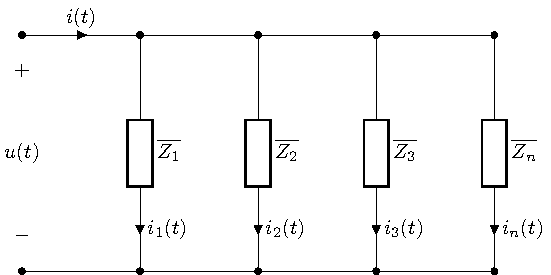
\includegraphics[height=4cm]{../figs/paralelo_general.pdf}\label{fig.paralelo-general-inicio}}\hfil
		\subfloat[Equivalente]{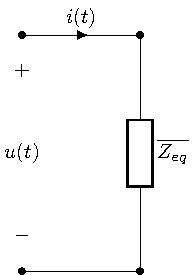
\includegraphics[height=4cm]{../figs/paralelo_general_eq.pdf}\label{fig.paralelo-general-eq}}
		\caption{Circuito paralelo general alimentado por corriente alterna}
		\label{fig.paralelo-general}
	\end{figure}
	
	Para el caso de circuitos en paralelo, se analiza directamente el circuito general. 
	%
	%\subsection{Circuito paralelo general}
	Considérese un circuito en paralelo formado por $n$ impedancias, donde cada impedancia es de la forma $\overline{Z_i}=R_i+\mathrm{j}\,X_i$, como se muestra en la Figura~\ref{fig.paralelo-general-inicio}. Este circuito se alimenta con una tensión $u(t)$, de valor eficaz $U$, de manera que circula por cada impedancia una intensidad $i_i(t)$ obtenidas según: 
	\begin{equation*}
		\overline{I_i}=\dfrac{\overline{U}}{\overline{Z_i}}
	\end{equation*}
	cumpliéndose, según la 1LK, que:
	\begin{equation*}
		\overline{I}=\overline{I_1}+\overline{I_2}+\overline{I_3}+...+\overline{I_n}
	\end{equation*}
	Por tanto, la corriente total $\overline{I}$ es:
	\begin{equation*}
		\overline{I}=\overline{I_1}+\overline{I_2}+\overline{I_3}+...+\overline{I_n}=\overline{U} \cdot\left(\dfrac{1}{\overline{Z_1}}+\dfrac{1}{\overline{Z_2}}+\dfrac{1}{\overline{Z_3}}+...+\dfrac{1}{\overline{Z_n}}\right)
	\end{equation*}
	Se dice que la impedancia equivalente a las $n$ impedancias en paralelo es aquella que, al aplicarle la misma tensión $u(t)$, origina la misma intensidad $i(t)$, es decir, la que \textbf{conserva el módulo de $\overline{I}$ y el ángulo de fase} entre $\overline{U}$ e $\overline{I}$ del circuito paralelo original. Puesto que en el circuito equivalente se cumple que: 
	\begin{equation*}
		\overline{I}=\dfrac{\overline{U}}{\overline{Z_{eq}}}
	\end{equation*}
	se llega a la conclusión de que:
	\begin{equation}
		\dfrac{1}{\overline{Z_{eq}}}=\dfrac{1}{\overline{Z_1}}+\dfrac{1}{\overline{Z_2}}+\dfrac{1}{\overline{Z_3}}+...+\dfrac{1}{\overline{Z_n}}\Rightarrow \boxed{\dfrac{1}{\overline{Z_{eq}}}=\dfrac{1}{\displaystyle\sum_{i=1}^n \overline{Z_i}}}
	\end{equation}
	
	\subsection{Admitancia}
	
	Puesto que el cálculo de la impedancia equivalente operando de esta forma es, con frecuencia, complicado y no exento de errores, es más frecuente hablar de \textbf{admitancia}. Conceptualmente, la admitancia representa la \textit{facilidad} que ofrece el circuito al paso de la corriente alterna, y es el recíproco (inversa) de la impedancia: 
	\begin{equation*}
	    \overline{Y}=\dfrac{1}{\overline{Z}}=\dfrac{1\phase{0^\circ}}{Z\phase{\theta^\circ}}=\dfrac{1}{Z}\phase{-\theta^\circ}=Y\phase\psi^\circ=G+\mathrm{j}\,B
	\end{equation*}
	donde $G$ es la conductancia y $B$ es la susceptancia. En función del valor de $B$, se tienen tres casos (al igual que con las impedancias):
	\begin{itemize}
		\item $B>0$: admitancia capacitiva
		\item $B<0$: admitancia inductiva
		\item $B=0$: admitancia resistiva
	\end{itemize}
	En los elementos simples, las admitancias se pueden calcular como: 
	\begin{align}
		\Aboxed{\overline{Y_R}&=\dfrac{1}{R}=G}\Rightarrow G\geq 0\\
		\Aboxed{\overline{Y_L}&=\dfrac{1}{\overline{X_L}}=\dfrac{1}{\mathrm{j}\,\omega\,L}=\dfrac{-\mathrm{j}}{\omega\,L}=B_L}\Rightarrow B_L\leq 0\\
		\Aboxed{\overline{Y_C}&=\dfrac{1}{\overline{X_C}}=\dfrac{1}{\frac{1}{\mathrm{j}\,\omega\,C}}=\mathrm{j}\,\omega\,C=B_C}\Rightarrow B_C\geq 0
	\end{align}
	Las admitancias se asocian en serie y paralelo de la misma forma que las impedancias, pero el cálculo de su valor equivalente es justo a la inversa: es decir, en paralelo su equivalente es la suma de las admitancias, y en serie el inverso de la admitancia equivalente es la suma de los inversos de las admitancias.
	
	\begin{figure}[H]
		\centering
		\subfloat[Impedancia]{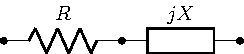
\includegraphics{../figs/Z.pdf}}\hfil
		\subfloat[Admitancia]{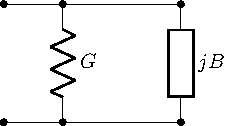
\includegraphics{../figs/Y.pdf}}
		\caption{Equivalencias entre impedancia y admitancia}
		\label{fig.equivalencias_impedancia_admitancia}
	\end{figure}
	De la Figura~\ref{fig.equivalencias_impedancia_admitancia}, se extraen las siguientes relaciones para que impedancia y admitancia sean equivalentes (es decir, se cumpla la igualdad $\overline{Z}\cdot \overline{Y}=1$): 
	\begin{equation}\label{eq.impedancia-admitancia}
		R+\mathrm{j}\,X=\dfrac{1}{G+\mathrm{j}\,B}=\frac{G-\mathrm{j}\,B}{(G+\mathrm{j}\,B)(G-\mathrm{j}\,B)}=\frac{G-\mathrm{j}\,B}{G^2+B^2} \Rightarrow 
		\boxed{\begin{cases}
				R=\dfrac{G}{G^2+B^2}\\[6pt]
				X=-\dfrac{B}{G^2+B^2}
		\end{cases}}
	\end{equation}
	\begin{equation}\label{eq.admitancia-impedancia}
		G+\mathrm{j}\,B=\dfrac{1}{R+\mathrm{j}\,X}=\dfrac{R-\mathrm{j}\,X}{(R+\mathrm{j}\,X)(R-\mathrm{j}\,X)}=\dfrac{R-\mathrm{j}\,X}{R^2+X^2} \Rightarrow 
		\boxed{\begin{cases}
				G=\dfrac{R}{R^2+X^2}\\[6pt]
				B=-\dfrac{X}{R^2+X^2}
		\end{cases}}
	\end{equation}
	
	
	\begin{remark}
		Las dimensiones de la admitancia y sus componentes son la inversa de $\Omega$ [S].
	\end{remark}
	
	La Figura~\ref{fig.impedancia_admitancia} muestra gráficamente una impedancia $\overline{Z}=R+\mathrm{j}\,X=Z\phase{\theta}$, donde su admitancia correspondiente es $\overline{Y}=G-\mathrm{j}\,B=Y\phase{-\psi}$.
	\begin{figure}[H]
		\centering
		\subfloat[Impedancia]{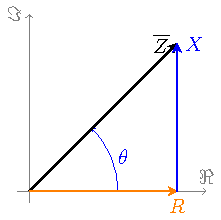
\includegraphics{../figs/impedancia.pdf}}\hfil
		\subfloat[Admitancia]{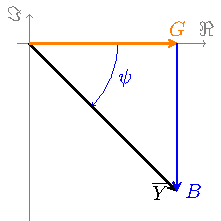
\includegraphics{../figs/admitancia.pdf}}
		\caption{Representación gráfica de la impedancia y admitancia}
		\label{fig.impedancia_admitancia}
	\end{figure}
	A partir de este gráfico, se pueden verificar las siguientes relaciones: 
	\begin{align*}
		Z=\sqrt{R^2+X^2}\qquad & \qquad Y=\sqrt{G^2+B^2}\\
		\theta=\arctan\left(\dfrac{X}{R}\right)\qquad &  \qquad \psi=\arctan\left(\dfrac{B}{G}\right)\\
		R=Z\cdot \cos(\theta)\qquad & \qquad G=Y\cdot \cos(\psi)\\
		X=Z\cdot \sin(\theta)\qquad & \qquad B=Y\cdot \sin(\psi)
	\end{align*}
	
	\begin{remark}
		Nótese que la susceptancia $B$ \textbf{siempre} tiene signo contrario a la reactancia $X$:
		\begin{align*}
			\text{Circuito inductivo}&: X > 0 \Rightarrow B<0\\
			\text{Circuito capacitivo}&: X < 0 \Rightarrow B>0
		\end{align*}
	\end{remark}
	
	\begin{example}\label{ex.impedancia_admitancia_eq}
	    \textbf{Calcular la impedancia y admitancia compleja equivalentes del circuito de la Figura~\ref{fig.impedancia_admitancia_eq}.}
	    \begin{figure}[H]
	        \centering
	        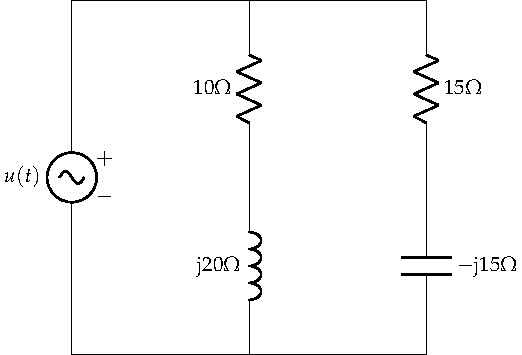
\includegraphics{../figs/impedancia_admitancia_eq.pdf}
	        \caption{Ejemplo~\ref{ex.impedancia_admitancia_eq}}
	        \label{fig.impedancia_admitancia_eq}
	    \end{figure}
	    
	    La impedancia equivalente de la resistencia y la bobina es:
	    \begin{equation*}
	        \overline{Z}_{R,L}=R+\overline{X}_L=10+\mathrm{j}20\,\Omega
	    \end{equation*}
	    y la de la resistencia y el condensador: 
	    \begin{equation*}
	        \overline{Z}_{R,C}=R+\overline{X}_C=15-\mathrm{j}15\,\Omega
	    \end{equation*}
	    siendo por tanto la impedancia equivalente total: 
	    \begin{equation*}
	        \overline{Z}_{eq}=\dfrac{1}{\dfrac{1}{\overline{Z}_{R,L}}+\dfrac{1}{\overline{Z}_{R,C}}}= \dfrac{1}{\dfrac{1}{10+\mathrm{j}20}+\dfrac{1}{15-\mathrm{j}15}}=18.61\phase{7.1250^\circ}\,\Omega
	    \end{equation*}
	    
	    A partir de la impedancia equivalente se determina la admitancia: 
	    \begin{equation*}
	        \overline{Y}_{eq}=\dfrac{1}{\overline{Z}_{eq}}=\dfrac{1}{18.61\phase{7.1250^\circ}}=0.05\phase{-7.1250^\circ}\,\si{\siemens}
	    \end{equation*}
	\end{example}
	
	\subsection{Antirresonancia}
	En un circuito paralelo $RLC$ se dice que se produce \textbf{antirresonancia} cuando la susceptancia es nula:
	\begin{equation*}
		B=\omega\,C-\dfrac{1}{\omega\,L}=0\rightarrow \omega\,C=\dfrac{1}{\omega\,L}
	\end{equation*}
	Por tanto, cuando se produce resonancia, se tiene que $\overline{Y}=G$, siendo un circuito resistivo puro. Como en el caso de la resonancia, se puede llegar a la antirresonancia variando la autoinducción $L$, la capacidad $C$ o la pulsación $\omega$. La pulsación $\omega_0$ necesaria para que se produzca antirresonancia, manteniendo constantes $L$ y $C$ es:
	\begin{equation}
		\omega_0\,C=\dfrac{1}{\omega_0\,L}\rightarrow \boxed{\omega_0=\dfrac{1}{\sqrt{L\,C}}}
	\end{equation}
	\begin{remark}
		Que la susceptancia $B$ tenga un valor nulo, no implica que la corriente en la bobina y el condensador sean 0. De hecho, pueden presentarse corrientes elevadas en éstos.
	\end{remark}
	
	\vspace{4mm}
	\begin{example}\label{ej.2-5}
		\textbf{Un circuito en paralelo formado por $R=1\,\Omega$, ${X_L}=0.01\,\Omega$ y ${X_C}=100\,\Omega$ se conecta a una tensión alterna $\overline{U}=100\phase{0^\circ}$ V. Calcular las corrientes de cada uno de los elementos.}
		
		En primer lugar, se calculan la conductancia de la resistencia y las susceptacias de bobina y condensador: 
		\begin{align*}
			\overline{G}&=\dfrac{1}{R}=\dfrac{1}{1}=1\;\text{S}\\
			\overline{B_L}&=-\dfrac{\mathrm{j}}{X_L}=-\dfrac{\mathrm{j}}{0.01}=-\mathrm{j}\,100\;\text{S}\\
			\overline{B_C}&=\mathrm{j}\,X_C=\mathrm{j}\,100\;\text{S}
		\end{align*}
		
		La susceptancia total se calcula como:
		\begin{equation*}
			\overline{B}= \overline{B_L}+\overline{B_C}=-\mathrm{j}\,100+\mathrm{j}\,100=0
		\end{equation*}
		
		Se trata de un circuito antirresonante, siendo la admitancia equivalente:
		\begin{equation*}
			\overline{Y}=G+\mathrm{j}\,B=1+\mathrm{j}\,0=1\;\text{S}
		\end{equation*}
		
		La corriente en cada elemento es:
		\begin{align*}
			\overline{I_R}&=\overline{G}\cdot \overline{U}={1\phase{0^\circ}}\cdot {100\phase{0^\circ}}=100\phase{0^\circ}\;\text{A}\\
			\overline{I_L}&=\overline{B_L}\cdot\overline{U}=100\phase{-90^\circ}\cdot 100\phase{0^\circ}=10000\phase{-90^\circ}\,\text{A}\\
			\overline{I_C}&=\overline{B_C}\cdot\overline{U}=100\phase{90^\circ}\cdot 100\phase{0^\circ}=10000\phase{90^\circ}\,\text{A}
		\end{align*}
	\end{example}
	
	
	
% 	\section{Componentes activa y reactiva de la intensidad}
% 	%Para explicar estos conceptos, se va a hacer referencia a las Secciones~\ref{sec.RL} y \ref{sec.RC}. 
	
% 	Considérese un circuito inductivo $RL$, es decir, la impedancia $\overline{Z}$ tiene un ángulo $\theta>0^\circ$ (Figura~\ref{fig.Z_ind_corriente}). Tomando como referencia la corriente $\overline{I}=I\phase{0^\circ}$, las tensiones en la resistencia ($U_R=R\cdot I$), bobina ($U_L=X\cdot I$) y total ($U=Z\cdot I$) se pueden representar en un diagrama fasorial como se muestra en la Figura~\ref{fig.tension_z_ind}. Por último, en la Figura~\ref{fig.corriente_z_ind}, se considera como referencia de fases la tensión $\overline{U}=U\phase{0^\circ}$, y se dibuja la corriente $\overline{I}$ que, como puede apreciarse, va \textbf{en retraso} respecto a la tensión (al tratarse de un circuito inductivo). 
	
% 	\begin{figure}[H]
% 		\centering
% 		\subfloat[Impedancias]{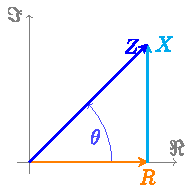
\includegraphics[height=4cm]{../figs/Z_ind_corriente.pdf}\label{fig.Z_ind_corriente}}\hfill
% 		%\subfloat[Admitancias]{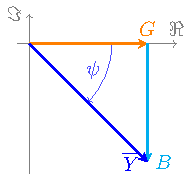
\includegraphics[width=0.25\linewidth]{../figs/Y_ind_corriente.pdf}}\hfil
% 		\subfloat[Tensiones ($\overline{I}=I\phase{0^\circ}$)]{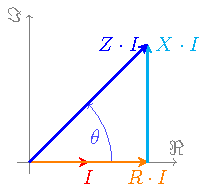
\includegraphics[height=4cm]{../figs/tension_Z_ind.pdf}\label{fig.tension_z_ind}}\hfill
% 		\subfloat[Corrientes ($\overline{U}=U\phase{0^\circ}$)]{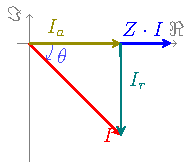
\includegraphics[height=3.6cm]{../figs/corriente_Z_ind.pdf}\label{fig.corriente_z_ind}}\hfil
% 		\caption{Diagramas fasoriales de un circuito inductivo $RL$}
% 		\label{fig.fasores_inductivo_corrientes}
% 	\end{figure}
	
% 	Ahora, considérese un circuito capacitivo $RC$, donde la impedancia $\overline{Z}$ tiene un ángulo $\theta<0^\circ$ (Figura~\ref{fig.Z_cap_corriente}). Tomando como referencia la corriente $\overline{I}=I\phase{0^\circ}$, las tensiones en la resistencia ($U_R=R\cdot I$), condensador ($U_C=X\cdot I$) y total ($U=Z\cdot I$) se pueden representar en un diagrama fasorial como se muestra en la Figura~\ref{fig.tension_z_cap}. Por último, en la Figura~\ref{fig.corriente_z_cap}, se considera como referencia de fases la tensión $\overline{U}=U\phase{0^\circ}$, y se dibuja la corriente $\overline{I}$ que, como puede apreciarse, va \textbf{en adelanto} respecto a la tensión (al tratarse de un circuito capacitivo). 
% 	\begin{figure}[H]
% 		\centering
% 		\subfloat[Impedancias]{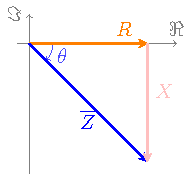
\includegraphics[height=4cm]{../figs/Z_cap_corriente.pdf}\label{fig.Z_cap_corriente}}\hfill
% 		%\subfloat[Admitancias]{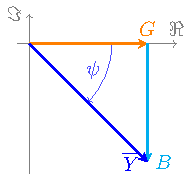
\includegraphics[width=0.25\linewidth]{../figs/Y_ind_corriente.pdf}}\hfil
% 		\subfloat[Tensiones ($\overline{I}=I\phase{0^\circ}$)]{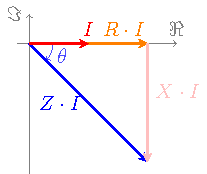
\includegraphics[height=4cm]{../figs/tension_Z_cap.pdf}\label{fig.tension_z_cap}}\hfill
% 		\subfloat[Corrientes ($\overline{U}=U\phase{0^\circ}$)]{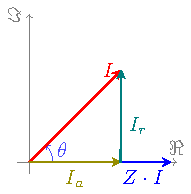
\includegraphics[height=4.4cm]{../figs/corriente_Z_cap.pdf}\label{fig.corriente_z_cap}}\hfil
% 		\caption{Diagramas fasoriales de un circuito capacitivo $RC$}
% 		\label{fig.fasores_capacitivo_corrientes}
% 	\end{figure}
	
% 	Como puede observarse, al dibujar el diagrama fasorial, cuando la tensión se considera como referencia $\overline{U}=U\phase{0^\circ}$ (Figuras~\ref{fig.corriente_z_ind} y \ref{fig.corriente_z_cap}), la corriente $\overline{I}$ puede descomponerse en dos:
% 	\begin{itemize}
% 		\item $I_a$, conocida como la  \textbf{componente activa} de la intensidad $\overline{I}$, que está \textbf{en fase} con la tensión $\overline{U}$
% 		\item $I_r$, conocida como la \textbf{componente reactiva} de la intensidad $\overline{I}$, que está \textbf{en cuadratura} con la tensión $\overline{U}$
% 	\end{itemize}
	
% 	\begin{remark}
% 		Nótese que no es necesario que $\overline{U}$ sea el origen de fases, como se muestra en la Figura~\ref{fig.corrientes_act_react}, ya que: $\overline{I}=\overline{I_a}+\overline{I_r}$
% 	\end{remark}
	
% 	\begin{figure}[H]
% 		\centering
% 		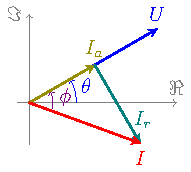
\includegraphics{../figs/corrientes_act_react.pdf}
% 		\caption{Componentes activa y reactiva de la corriente}
% 		\label{fig.corrientes_act_react}
% 	\end{figure}
	
% 	Del diagrama de la Figura~\ref{fig.corrientes_act_react} se deduce que: 
% 	\begin{equation*}
% 		\overline{U}=U\phase{\theta}\Rightarrow \overline{I}=I\phase{\theta-\phi}=I\cos(\phi)\phase{\theta}+I\sin(\phi)\phase{\phi-\frac{\pi}{2}}
% 	\end{equation*}
% 	que en el caso particular de que $\overline{U}=U\phase{0}$:
% 	\begin{equation*}
% 		\overline{I}=I_a+\mathrm{j}\,I_r=I\cos(\theta)-\mathrm{j}\,I\sin(\theta)
% 	\end{equation*}
% 	donde $I_r$ \textbf{tiene signo contrario} al de $\theta$ de la impedancia.
	
	\section{Potencia en corriente alterna}\label{sec.potencia_CA}
	
	Cuando se conecta una impedancia a una tensión alterna de expresión $u(t) = U\sqrt{2} \cdot\cos (\omega t)$, la impedancia es recorrida por una corriente:
	\begin{equation*}
		i(t) = I\sqrt{2} \cdot \cos (\omega t -\theta)
	\end{equation*}
	siendo $\theta>0$ si la impedancia es inductiva y $\theta<0$ si es capacitiva. La \textbf{potencia instantánea} entregada al circuito está definida por:
	\begin{equation*}
		p(t)=u(t)\cdot i(t)=\left(U\sqrt{2}\cdot \cos (\omega t) \right)\cdot \left(I\sqrt{2} \cdot \cos (\omega t -\theta)\right)=2\cdot U\cdot I\cdot \cos(\omega t)\cdot\cos(\omega t-\theta)
	\end{equation*}
	donde, teniendo en cuenta:
	\begin{align*}
		\cos(\alpha-\beta)&=\cos(\alpha)\cdot\cos(\beta)+\sin(\alpha)\cdot\sin(\beta)\\
		\cos(\alpha+\beta)&=\cos(\alpha)\cdot\cos(\beta)-\sin(\alpha)\cdot\sin(\beta)\\[-10pt]
		\cline{1-2}
		\cos(\alpha-\beta)+\cos(\alpha+\beta)&=2\cdot\cos(\alpha)\cdot\cos(\beta)%\rightarrow \sin(\alpha)\cdot\sin(\beta)=\dfrac{1}{2}\cdot \left[ \cos(\alpha-\beta)-\cos(\alpha+\beta)\right]
	\end{align*}
	y considerando como $\alpha=\omega t$ y $\beta=\omega t-\theta$:
	\begin{align*}
		\alpha-\beta&=\theta\\
		\alpha +\beta&=2\omega t-\theta
	\end{align*}
	por lo que la potencia instantánea resulta:
	\begin{equation}\label{eq.pot_inst}
		p(t)=2\cdot U\cdot I\cdot \overbrace{\cos(\omega t)}^{\cos(\alpha)}\cdot\overbrace{\cos(\omega t-\theta)}^{\cos(\beta)}\Rightarrow \boxed{p(t)
			=U\cdot I \cdot \cos(\theta)+U\cdot I \cdot\cos(2\omega t-\theta)}
	\end{equation}
	Según esta ecuación, la potencia instantánea consta de un {valor constante} (el primer término, $U\cdot I\cdot \cos(\theta)$) y una componente sinusoidal (el segundo término, $U\cdot I\cdot \cos(2 \omega t-\theta)$) de frecuencia $2\omega$ (\textbf{doble} de $u(t)$ o $i(t)$). Como puede verse en la Figura~\ref{fig.inductivoPuroPotencia}, $p(t)$ es negativa para los intervalos de tiempo en los que $u(t)$ e $i(t)$ tienen signos opuestos. En los periodos de tiempo en que la potencia es negativa, la impedancia \textbf{devuelve energía} a la red, algo que solo es posible si contiene elementos almacenadores de energía (es decir, bobinas o condensadores). 
	
	\begin{figure}[H]
		\centering
		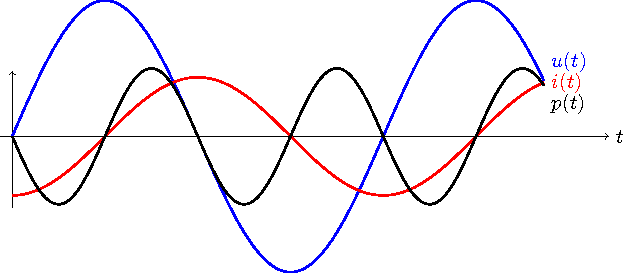
\includegraphics{../figs/inductivoPuroPotencia.pdf}
		\caption{Ondas de tensión, corriente y potencia instantáneas}
		\label{fig.inductivoPuroPotencia}
	\end{figure}
	
	Por tanto, la potencia instantánea cambia con el tiempo y es difícil de medir. Si se hace el valor medio de la expresión~\eqref{eq.pot_inst} en un periodo, mediante la ecuación~\eqref{eq.valor_medio}:
	\begin{equation*}
		P_m=\dfrac{1}{T}\int_{0}^{T}p(t)\,dt=\dfrac{1}{T}\int_{0}^{T}U\,I\,\cos(\theta)\,dt+\cancelto{0}{\dfrac{1}{T}\int_{0}^{T}U\,I\,\cos(2\omega t-\theta)\,dt}
	\end{equation*}
	siendo el primer integrando constante y el segundo integrando una sinusoide. Dado que el promedio de una sinusoide a lo largo de un periodo es nulo (el área bajo la sinusoide durante medio ciclo positivo es cancelada por el área bajo ella durante el siguiente medio ciclo negativo), este término se anula y la potencia promedio se convierte en $P=U\,I\,\cos(\theta)$, que coincide con el término fijo de $p(t)$ y es la \textbf{potencia real} consumida en los elementos disipativos de la impedancia. El término $-U\,I\,\cos(2\omega t-\theta)$ es el responsable de que $p(t)$ fluctúe (oscile) en torno a su valor medio ($P$); de ahí que se conozca como \textbf{potencia fluctuante}. Si se desarrolla $p(t)$ teniendo en cuenta la relación para el coseno de una resta, resulta: 
	\begin{align*}
		p(t)&=U\,I\,\cos(\theta)+U\,I\,\cos(\overbrace{2\omega\,t}^{\alpha}-\overbrace{\theta}^{\beta})=U\,I\,\cos(\theta)+\left[ U\,I\,\cos(\theta)\,\cos(2\omega t) + U\,I\sin(\theta)\,\sin(2\omega t)\right]=\\
		&=\underbrace{{\color{blue}U\,I\,\cos(\theta)}\left[1+\cos(2\omega t)\right]}_{p_1(t)} + \underbrace{{\color{red}U\,I\sin(\theta)}\,\sin(2\omega t)}_{p_2(t)}={\color{blue}P}\left[1+\cos(2\omega t)\right] + {\color{red}Q}\,\sin(2\omega t)
	\end{align*}
	Por tanto, la potencia eléctrica instantánea absorbida por una impedancia consta de dos términos variables en el tiempo con frecuencia $2\omega$:
	\begin{itemize}
		\item $p_1(t)$, positivo y oscilante en torno al valor medio $P=U\,I\,\cos(\theta)$. Es la potencia instantánea que consumen los elementos resistivos, y se denomina \textbf{potencia activa} [W]:
		\begin{equation}
			\boxed{P=U\,I\,\cos(\theta)}
		\end{equation}
		\item $p_2(t)$, es la potencia instantánea que almacena o devuelve el circuito (no implica transformación en trabajo útil), razón por la que se denomina \textbf{potencia entretenida}. La máxima potencia que almacena/devuelve el circuito se identifica con la letra $Q$ y se denomina \textbf{potencia reactiva}. Al no ser ``potencia consumida'', para diferenciarla de $P$, su unidad se denomina \textbf{voltamperio reactivo} [VAr]:
		\begin{equation}
			\boxed{Q=U\,I\,\sin(\theta)}
		\end{equation}
	\end{itemize}
	
	\subsection{Circuito resistivo}\label{sec.potencia_R}
	Una resistencia, como ya se ha indicado en la Sección~\ref{sec.R-puro}, presenta una impedancia $\overline{Z_R}=R\phase{0^\circ}\rightarrow \theta=0^\circ$. Por tanto, las potencias activa y reactiva: 
	\begin{equation}
		\theta = 0 \rightarrow
		\boxed{\begin{cases}
				P = U\cdot I = \dfrac{U^2}{R} = I^2\cdot R\\
				Q = 0
		\end{cases}}
	\end{equation}
	puesto que $\cos(0^\circ)=1$ y $\sin(0^\circ)=0$. Dibujando las ondas de $u(t)$, $i(t)$ y $p(t)$ (Figura~\ref{fig.resistivoPotencia}), se observa que $p(t)$ fluctúa al doble de frecuencia que $u(t)$ e $i(t)$, y que \textbf{siempre es positiva}, puesto que tensión y corriente van en fase y, por tanto, siempre tienen el mismo signo. Además, su valor medio es igual a $P=U\cdot I$.
	\begin{figure}[H]
		\centering
		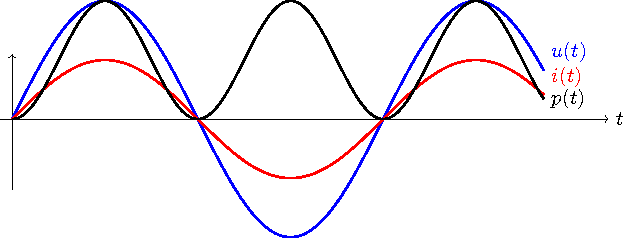
\includegraphics{../figs/resistivoPotencia.pdf}
		\caption{Ondas de tensión, corriente y potencia instantáneas en un circuito resistivo}
		\label{fig.resistivoPotencia}
	\end{figure}
	
	\subsection{Circuito inductivo puro}\label{sec.potencia_L}
	Una bobina, como ya se ha indicado en la Sección~\ref{sec.L-puro}, presenta una impedancia $\overline{Z_L}=\omega\cdot L\phase{90^\circ}\rightarrow \theta=90^\circ$. Por tanto, las potencias activa y reactiva: 
	\begin{equation}
		\theta = 90^\circ \rightarrow
		\boxed{\begin{cases}
				P = 0\\
				Q = U\cdot I = \dfrac{U^2}{\omega L} = I^2\cdot  \omega L
		\end{cases}}
	\end{equation}
	puesto que $\cos(90^\circ)=0$ y $\sin(90^\circ)=1$. Dibujando las ondas de $u(t)$, $i(t)$ y $p(t)$ (Figura~\ref{fig.inductivoPotencia}), se observa que $p(t)$ fluctúa al doble de frecuencia que $u(t)$ e $i(t)$, y que \textbf{tiene periodos positivos y negativos}, pasando por los ceros de tensión y corriente. Además, su valor medio es nulo, coincidiendo con $P=0$.
	\begin{figure}[H]
		\centering
		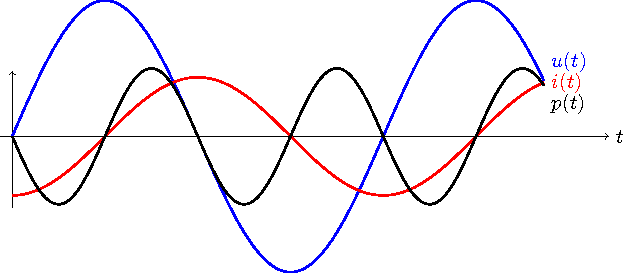
\includegraphics{../figs/inductivoPuroPotencia.pdf}
		\caption{Ondas de tensión, corriente y potencia instantáneas en un circuito inductivo puro}
		\label{fig.inductivoPotencia}
	\end{figure}
	
	\subsection{Circuito capacitivo puro}\label{sec.potencia_C}
	Un condensador, como ya se ha indicado en la Sección~\ref{sec.C-puro}, presenta una impedancia $\overline{Z_C}=\frac{1}{\omega\cdot C}\phase{-90^\circ}\rightarrow \theta=-90^\circ$. Por tanto, las potencias activa y reactiva: 
	\begin{equation}
		\theta = -90^\circ \rightarrow
		\boxed{\begin{cases}
				P = 0\\
				Q = -U\cdot I = -U^2\cdot \omega C = -\dfrac{I^2}{\omega C}
		\end{cases}}
	\end{equation}
	puesto que $\cos(-90^\circ)=0$ y $\sin(-90^\circ)=-1$. Dibujando las ondas de $u(t)$, $i(t)$ y $p(t)$ (Figura~\ref{fig.capacitivoPotencia}), se observa que $p(t)$ fluctúa al doble de frecuencia que $u(t)$ e $i(t)$, y que \textbf{tiene periodos positivos y negativos}, pasando por los ceros de tensión y corriente. Además, su valor medio es nulo, coincidiendo con $P=0$.
	\begin{figure}[H]
		\centering
		\includegraphics{../figs/capacitivoPuroPotencia.pdf}
		\caption{Ondas de tensión, corriente y potencia instantáneas en un circuito capacitivo puro}
		\label{fig.capacitivoPotencia}
	\end{figure}
	
	\subsection{Triángulo de potencias}
	Supóngase un circuito con carácter inductivo, con resistencia $R$ y reactancia $X$. El módulo de la impedancia global del circuito puede calcularse como $\overline{Z}=\sqrt{R^2+X^2}$, obteniendo un diagrama fasorial conocido como \textbf{triángulo de impedancias}. Si se multiplica cada lado de dicho triángulo por el módulo de $\overline{I}$, se obtiene el \textbf{triángulo de tensiones}, donde el eje $\Re$ es el módulo de la tensión en la resistencia $U_R=R\cdot I$ y el eje $\Im$ es el módulo de la tensión en la reactancia $U_X=X\cdot I$, siendo el módulo de la tensión total $U=Z\cdot I=\sqrt{U_R^2+U_X^2}$. Si, de nuevo, vuelve a multiplicarse dicho triángulo por el módulo de $\overline{I}$, se llega al \textbf{triángulo de potencias}, siendo el eje $\Re$ la potencia activa $P=R\cdot I^2$ y, el eje $\Im$, la potencia reactiva $Q=X\cdot I^2$. La hipotenusa de dicho triángulo es conocida como \textbf{potencia aparente}. Estos triángulos se presentan en la Figura~\ref{fig.triangulo_potencias}. 
	\begin{figure}[H]
		\centering
		\subfloat[Impedancias]{\includegraphics[height=4cm]{../figs/Z_ind_corriente.pdf}}\hfill
		\subfloat[Tensiones ]{\includegraphics[height=4cm]{../figs/tension_Z_ind.pdf}}\hfill
		\subfloat[Potencias]{\includegraphics[height=4cm]{../figs/triangulo_potencias.pdf}\label{fig.triangulo_potencias_pqs}}\hfil
		\caption{Triángulo de potencias de un circuito inductivo $RL$}
		\label{fig.triangulo_potencias}
	\end{figure}
	
	Se detalla a continuación el significado de cada una de las potencias representadas en el triángulo: 
	\begin{itemize}
		\item \textbf{Potencia activa.} Cateto contiguo en la Figura~\ref{fig.triangulo_potencias_pqs}. Suele denominarse únicamente como \textit{potencia}, al tratarse de la que es \textbf{realmente consumida} por el circuito. Su unidad es el [W]:
		\begin{equation}\label{eq.Pactiva}
			\boxed{P = U\cdot I\cdot\cos(\theta) = R \cdot I^2}
		\end{equation}
		\item \textbf{Potencia reactiva.} Cateto opuesto en la Figura~\ref{fig.triangulo_potencias_pqs}. Es el \textbf{valor máximo de la potencia entretenida} (almacenada y cedida) por los elementos almacenadores de energía (bobinas y condensadores). Se considera positiva $+$ si el circuito es inductivo ($\theta>0^\circ$) y negativa $-$ si el circuito es capacitivo ($\theta<0^\circ$). Su unidad es el [VAr] y se calcula mediante: 
		\begin{equation}\label{eq.Qreactiva}
			\boxed{Q = U\cdot I\cdot\sin(\theta) = X \cdot I^2}
		\end{equation}
		\item \textbf{Potencia aparente.} Hipotenusa en la Figura~\ref{fig.triangulo_potencias_pqs}. No es ``potencia consumida'' en sentido estricto (excepto cuando $\cos(\theta)=1$), pero representa la \textbf{potencia demandada} al generador/red; se denomina \textit{potencia aparente}, puesto que es la potencia que, ``en apariencia'', la red entrega a las cargas. Para diferenciarla de $P$ y $Q$, su unidad es el \textbf{voltamperio} [VA] y puede expresarse como: 
		\begin{equation}\label{eq.Saparente}
			\boxed{S = U\cdot I= Z \cdot I^2=\sqrt{P^2+Q^2}}
		\end{equation}
		donde la última igualdad se obtiene al aplicar el teorema de Pitágoras a la Figura~\ref{fig.triangulo_potencias_pqs}. Además, se observa que puede expresarse también mediante un \textbf{número complejo} (al igual que $\overline{Z}$ y $\overline{U}$): 
		\begin{equation}
			\boxed{\overline{S}=P+\mathrm{j}\,Q=\overline{U}\cdot \overline{I^*}=S\phase{\theta}}
		\end{equation}
		conociéndose entonces como \textbf{potencia compleja}. La igualdad $\overline{S}=\overline{U}\cdot \overline{I^*}$ se obtiene, considerando que $\overline{U} = U\phase{0}$ y $\overline{I} = I\phase{-\theta}$, de la siguiente forma: 
		\begin{equation*}
			\overline{U} \overline{I}^* = U\phase{0} \cdot I\phase{\theta} = UI\phase{\theta}= U I (\cos\theta + \mathrm{j} \sin\theta) = P + \mathrm{j} Q
		\end{equation*}
		\begin{remark}
			Nótese que la fase de $\overline{S}$ es \textbf{igual} a la fase de la impedancia $\overline{Z}$:
			\begin{equation*}
				\theta_S = \theta_Z = \theta
			\end{equation*}
		\end{remark}
		La Figura~\ref{fig.trianguloPotencias} muestra la potencia compleja y su descomposición en $P$ y $Q$.
		\begin{figure}[H]
			\centering
			\includegraphics{../figs/trianguloPotencias.pdf}
			\caption{Triángulo de potencias}
			\label{fig.trianguloPotencias}
		\end{figure}
	\end{itemize}
	
	
	\subsection{Resumen de potencia de los elementos pasivos}
	
	Se presenta aquí un resumen de los tipos de potencia consumida por cada elemento pasivo básico: 
	\begin{itemize}
		\item \textbf{Resistencia:}
		\begin{equation*}
			\theta = 0^\circ \Rightarrow 
			\begin{cases}
				P_R = R I^2\\
				Q_R = 0\\
				\overline{S_R} = R I^2\phase{0^\circ}
			\end{cases}
		\end{equation*}
		
		
		
		\begin{itemize}
			\item Consume potencia activa
			\item No consume potencia reactiva
		\end{itemize}
		
		\item \textbf{Inductancia:}
		\begin{equation*}
			\theta = 90^\circ \Rightarrow 
			\begin{cases}
				P_L = 0\\
				Q_L = \omega L I^2\\
				\overline{S}_L = \omega L I^2 \phase{90^\circ}
			\end{cases}
		\end{equation*}
		
		
		\begin{itemize}
			\item No consume potencia activa
			\item Consume potencia reactiva ($Q > 0$)
		\end{itemize}
		
		\item \textbf{Condensador:}
		\begin{equation*}
			\theta = - 90^\circ \Rightarrow 
			\begin{cases}
				P_L = 0\\
				Q_C = - \omega C U^2\\
				\overline{S}_C = \omega C U^2 \phase{- 90^\circ}
			\end{cases}   
		\end{equation*}
		
		
		\begin{itemize}
			\item No consume potencia activa
			\item Genera potencia reactiva ($Q < 0$)
		\end{itemize}
		
		
	\end{itemize}
	
	\subsection{Teorema de Boucherot}\label{sec.boucherot}
	El teorema de Boucherot es una consecuencia del principio de
        conservación de la energía y, de hecho, puede encontrarse
        también como \textit{principio de conservación de la potencia
          compleja}. Se demuestra aquí para el caso de un circuito en
        serie.
	
	Sea un circuito en serie formado por 3 impedancias:
        $\overline{Z_1}=R_1+\mathrm{j}\,X_1$,
        $\overline{Z_2}=R_2+\mathrm{j}\,X_2$ y
        $\overline{Z_3}=R_3-\mathrm{j}\,X_3$ (es decir,
        $\overline{Z_1}$ y $\overline{Z_2}$ tienen carácter inductivo
        y $\overline{Z_3}$ tiene carácter capacitivo). Por comodidad,
        se supondrá que $\overline{I}=I\phase{0^\circ}$. Por la 2LK se
        cumple que:
	\begin{equation*}
          \overline{U}=\sum_{i=1}^3 \overline{U_i}\Rightarrow
          \begin{cases}
            U\,\cos(\theta)=\displaystyle\sum_{i=1}^3 U_i\,\cos(\theta_i)\\
            U\,\sin(\theta)=\displaystyle\sum_{i=1}^3 U_i\,\sin(\theta_i)
          \end{cases}
	\end{equation*}
	Multiplicando las dos expresiones anteriores por la corriente
        (la misma en todo el circuito, al tratarse de una conexión en
        serie), se obtienen las relaciones entre las potencias, que
        puede verse gráficamente en la Figura~\ref{fig.boucherot}:
	\begin{align*}
          U\,I\,\cos(\theta)&=P_T=\displaystyle\sum_{i=1}^3 U_i\,I\,\cos(\theta_i)=\displaystyle\sum_{i=1}^3 P_i=\displaystyle\sum_{i=1}^3 R_i\cdot I^2\\
          U\,I\,\sin(\theta)&=Q_T=\displaystyle\sum_{i=1}^3 U_i\,I\,\sin(\theta_i)=\displaystyle\sum_{i=1}^3 Q_i=\displaystyle\sum_{i=1}^3 X_i\cdot I^2\\
	\end{align*}
	\begin{figure}[H]
          \centering
          \includegraphics[width=0.7\linewidth]{../figs/boucherot.pdf}
          \caption{Teorema de Boucherot}
          \label{fig.boucherot}
	\end{figure}
	
	Es decir, se cumple que:
	\begin{itemize}
        \item La potencia activa total es la suma aritmética (suma de
          números naturales) de las potencias activas de cada receptor
        \item La potencia reactiva total es la suma algebraica (suma
          de números enteros, considerando el signo) de las potencias
          reactivas de cada receptor
	\end{itemize}
	Estas dos afirmaciones expresan el teorema de Boucherot, de
        manera que se cumple que la potencia activa y reactiva total
        es la suma de las potencias activas y reactivas individuales
        (respectivamente) y, por tanto, que la potencia compleja total
        es la suma de las potencias aparentes individuales:
	\begin{equation}\label{eq.S_compleja_mono}
          \boxed{\overline{S} =P+\mathrm{j}\,Q= \sum^n_{i = 1} (P_i + jQ_i)=\sum_{i = 1}^{n} \overline{S}_i}
	\end{equation}
	
	\vspace{4mm}
	\begin{example}\label{ej.2-7}
          \textbf{Sabiendo que las fuentes de tensión del circuito de
            la Figura \ref{fig.problema9_garri} vienen definidas por
            las formas de onda
            $u_1(t)=10\sqrt{2}\cdot \cos(1000\cdot t) \,\si{\volt}$ y
            $u_2(t)=5\sqrt{2}\cdot \sin(1000\cdot t) \,\si{\volt}$, calcular las
            potencias de cada elemento, así como el balance de
            potencias del circuito. }
          \begin{figure}[H]
            \centering
            \includegraphics[width=0.6\linewidth]{../figs/ej7_BT2.pdf}
            \caption{Ejemplo \ref{ej.2-7}}
            \label{fig.problema9_garri}
          \end{figure}
		
          Se convierte $u_1(t)$ en función senoidal, obteniéndose
          $u_1(t)=10\sqrt{2}\cdot \sin(1000\cdot
          t+\frac{\pi}{2}) \,\si{\volt}$. Así, los fasores de $\overline{U}_1$ y
          $\overline{U}_2$ son:
          \begin{align*}
            \overline{U}_1&=10\phase{90^\circ}\,\si{\volt}\\
            \overline{U}_2&=5\phase{0^\circ}\,\si{\volt}
          \end{align*}
		
          Se calcula también el valor de $\overline{X}_L$:
          \begin{equation*}
            \overline{X}_L=\mathrm{j}\,\omega L=\mathrm{j}\,\Omega
          \end{equation*}
		
          Con esto, el sistema matricial por el método de mallas es:
          \begin{equation*}
            \begin{bmatrix}
              \vphantom{\dfrac{1}{1}}10\phase{90^\circ} \\[4pt]
              \vphantom{\dfrac{1}{1}}5\phase{180^\circ} 
            \end{bmatrix}
            =
            \begin{bmatrix}
              \vphantom{\dfrac{1}{1}}1-\mathrm{j}\,2 & \quad\mathrm{j}\,2 \\[4pt]
              \vphantom{\dfrac{1}{1}}\mathrm{j}\,2 & -\mathrm{j} \\
            \end{bmatrix}
            \cdot 
            \begin{bmatrix}
              \vphantom{\dfrac{1}{1}}\overline{I}_a\\[4pt]
              \vphantom{\dfrac{1}{1}}\overline{I}_b
            \end{bmatrix}
          \end{equation*}          
          donde el valor de $5\phase{\ang{180}}$ resulta de tomar el negativo del fasor $\overline{U}_2$, dado que la corriente de malla $\overline{I}_b$ ``entra'' por el polo $+$ de la fuente $u_2$ (tomar el negativo de un número complejo en forma polar equivale a adelantar su ángulo en $180^\circ$)

          \vspace{3mm}
          Resolviendo el sistema, se obtiene:
          \begin{align*}
            \overline{I}_a&= 2 + 6\mathrm{j}\,\unit{\ampere}\\
            \overline{I}_b&= 4 + 7\mathrm{j}\,\unit{\ampere}
          \end{align*}          
          y reemplazando en el circuito:
          \begin{align*}
            \overline{I}&=\overline{I}_a= 2 + 6\mathrm{j}\,\unit{\ampere}\\
            \overline{I}_1&=\overline{I}_a - \overline{I}_b= -2 -\mathrm{j}\,\unit{\ampere}\\
            \overline{I}_2&=-\overline{I}_b= -4 - 7\mathrm{j}\,\unit{\ampere}\\
          \end{align*}	

          \vspace{-3mm}
          Con las corrientes y los valores de las impedancias, se
          calculan las potencias activas y reactivas en los elementos pasivos:
          \begin{align*}
            P_R&=R\cdot I^2=\qty{40}{\watt}\\
            Q_L &= X_L\cdot I_2^2=\qty{65}{\voltamperer}\\
            Q_C&=X_C\cdot I_1^2=-\qty{10}{\voltamperer}
          \end{align*}
          siendo la potencia aparente total consumida por los
          receptores:
          \begin{equation*}
            \overline{S}=P+\mathrm{j}\,Q= 40 + 55\mathrm{j}\,\unit{\voltampere}
          \end{equation*}
		
          Se calcula también la potencia aparente entregada por las
          fuentes de alimentación:
          \begin{align*}
            \overline{S}_{u1}&=\overline{U}_1\cdot \overline{I}^*= 60 + 20\mathrm{j}\,\unit{\voltampere}\\
            \overline{S}_{u2}&=\overline{U}_2\cdot \overline{I}_2^*= -20 + 35\mathrm{j}\,\unit{\voltampere}\\
            \overline{S}_g &= \overline{S}_{u1} + \overline{S}_{u2} = 40 + 55\mathrm{j}\,\unit{\voltampere}
          \end{align*}
          Comprobamos que coincide con el triángulo de potencias de los receptores.
                        
	\end{example}
	
	\subsection{Medida de potencia: vatímetro}\label{sec.medida_potencia}
	
	La medida de potencia activa y reactiva es de gran importancia para determinar el comportamiento de los circuitos de corriente alterna. La expresión de la potencia activa $P$ se corresponde con la \textbf{parte real} de la potencia aparente compleja, según se indicó en la expresión~\eqref{eq.S_compleja_mono}. Para medir $P$, se utiliza un instrumento de medida denominado \textbf{vatímetro}, puesto que, debido al $\cos(\theta)$, no es posible hacerlo únicamente con voltímetro y amperímetro. El vatímetro es un equipo que consta de dos bobinas (una de intensidad, o circuito amperimétrico; y otra de tensión, o circuito voltimétrico) y, por tanto, cuatro terminales (dos para la tensión y otros dos para la corriente, como se muestra en la Figura~\ref{fig.vatimetro_2}), cuya lectura da como resultado directamente el valor de la potencia:
	\begin{equation*}
	    W=\Re(\overline{U}_{3,4} \cdot \overline{I}_{1,2}^*)=I_{1,2}\cdot U_{3,4}\cdot \cos\widehat{(I_{1,2}, U_{3,4})}
	\end{equation*}%En la actualidad, hay aparatos digitales de medida que captan la tensión y la intensidad y, con estas muestras, pueden obtenerse las potencias activas y reactivas, así como otras magnitudes. Sin embargo, los medidores analógicos de potencia activa y reactiva se siguen utilizando ampliamente. 
	
	\begin{figure}[H]
	    \centering
	    \includegraphics{../figs/vatimetro_2.pdf}
	    \caption{Conexiones del vatímetro}
	    \label{fig.vatimetro_2}
	\end{figure}
	Considerando las bornas 1 y 3 como entradas, si el ángulo formado por $\overline{I_{1,2}}$ y $\overline{U_{3,4}}$ es menor que $90^\circ$ o mayor que $270^\circ$, el valor de $\cos\widehat{(I_{1,2}, U_{3,4})}$ será positivo. Pero si el ángulo es mayor que $90^\circ$ o menor de $270^\circ$, el valor de  $\cos\widehat{(I_{1,2}, U_{3,4})}$ será negativo y el vatímetro tratará de marcar en sentido contrario, clavándose en $0$ la aguja (en caso de ser analógico) o apareciendo el signo $-$ (en los digitales). En ese caso, basta con invertir las conexiones en uno de los dos circuitos (generalmente el de tensión, por no cortar la continuidad de la alimentación a los receptores) para obtener una lectura positiva. No obstante, deberá considerarse esta lectura como \textbf{negativa} a efectos del cómputo de la potencia total. 
	
	
	\subsection{Factor de potencia: importancia y mejora}\label{sec.mejora_fdp_monofasica}
	
	El factor de potencia, $fdp$ o $\cos(\theta)$, representa la aportación de potencia activa dentro de la potencia aparente:
	\begin{equation}
		\boxed{\cos(\theta)=\dfrac{P}{S}}
	\end{equation}
	y es igual al coseno del ángulo entre $\overline{U}$ e $\overline{I}$. Se dice que:
	\begin{itemize}
		\item $\cos(\theta)$ es \textbf{en retraso} cuando el circuito tiene carácter inductivo (la intensidad va retrasada respecto a la tensión)
		\item $\cos(\theta)$ es \textbf{en adelanto} cuando el circuito tiene carácter capacitivo (la intensidad va adelantada respecto a la tensión)
	\end{itemize}
	\begin{remark}
		Como $\cos(\theta)\leq 1$, su valor supone un límite a la potencia activa que se puede consumir en una instalación: ésta será máxima para $\cos(\theta)=1\Rightarrow \theta=0^\circ$ pero, para cualquier otro valor de $\theta$, aún con los mismos valores de $U$ e $I$, la potencia activa consumida será inferior. 
	\end{remark}
	
	Sean dos sistemas con la \textbf{misma tensión y potencia activa}, pero con diferentes factores de potencia $\cos(\theta_2) < \cos(\theta_1)$, lo que implica que $Q_2 > Q_1$ (Figura~\ref{fig.fasorescompensacionreactiva}). Se observa que el sistema 2 requiere una \textbf{mayor potencia aparente} (es decir, un generador mayor) para alimentar la misma potencia activa:
	\begin{equation*}
		\left(\dfrac{P}{\cos(\theta_1)} = S_1 \right) < \left( S_2 = \dfrac{P}{\cos (\theta_2)}\right) 
	\end{equation*}
	Además, el sistema 2 requiere también una \textbf{mayor sección} de cable para transportar la misma potencia activa, dado que la sección del conductor está relacionada con la intensidad que circula por él; esto implica un coste adicional en la instalación:
	\begin{equation*}
		\left(\frac{P}{U \cos (\theta_1)} = I_1 \right) < \left( I_2 = \frac{P}{U \cos (\theta_2)}\right) 
	\end{equation*}
	\begin{figure}[H]
		\centering
		\includegraphics{../figs/fasorescompensacionreactiva.pdf}
		\caption{Fasores de potencias para dos sistemas con $U$ y $P$, pero diferentes $\cos(\theta)$}
		\label{fig.fasorescompensacionreactiva}
	\end{figure} 
	
	Todo ello hace que las compañías suministradoras penalicen a los consumidores que tienen factores de potencia bajos, haciéndoles pagar una tasa adicional. De hecho, en determinados casos, se obliga a instalar elementos que mejoren dicho factor de potencia (aumenten a $\cos(\theta)\approx 1$). Dado que la mayoría de los receptores tienen un \textbf{carácter inductivo} (máquinas eléctricas industriales), para mejorar el $\cos(\theta)$ se conectan \textbf{bancos de condensadores} en paralelo con los receptores hasta lograr el factor de potencia deseado.
	
	Sea una carga de potencia activa $P_Z$, potencia reactiva $Q_Z$ y factor de potencia $\cos(\theta)$, a la que se le quiere \textbf{mejorar el factor de potencia} de manera que $\cos (\theta') > \cos (\theta)$, pero manteniendo el valor de $P_Z$. Así, hay que introducir \textbf{en paralelo} una capacidad $C$ capaz de generar un valor $Q_C$ que compense la reactiva inicial $Q_Z$ hasta el valor deseado $Q'$. Se cumple entonces que: 
	\begin{align*}
		P' &= P_Z\\
		Q' &= Q_C + Q_Z \quad (Q_C<0\Rightarrow Q' < Q_Z)\\
		\overline{I'} &= \overline{I_C} + \overline{I_Z}
	\end{align*}
	donde las magnitudes con $'$ hacen referencia a la situación una vez introducido el condensador (ver Figura~\ref{fig.circuito_compensacion}). A partir del triángulo de potencias (Figura~\ref{fig.triangulocompensacionQ}) se deduce que:
	\begin{align*}
		Q_Z &= P_Z \tan (\theta)\\
		Q'&= P_Z \tan (\theta')
	\end{align*}
	\begin{equation}\label{eq.compensacion_Q_mono}
		|Q_C| = Q_Z - Q' = P_Z\cdot \left[\tan (\theta) - \tan (\theta')\right]=\dfrac{U^2}{X_C}={U^2\,\omega\,C}\rightarrow \boxed{C=\frac{P_Z \left[\tan (\theta) - \tan (\theta')\right]}{\omega U^2}}
	\end{equation}
	
	
	\begin{figure}
		\centering
		\subfloat[Circuito]{\includegraphics[height=3cm]{../figs/circuitocompensacionreactiva.pdf}\label{fig.circuito_compensacion}}
		\hfil
		\subfloat[Triángulo de potencias]{\includegraphics{../figs/trianguloCompensacionQ.pdf}\label{fig.triangulocompensacionQ}}
		\caption{Circuito de compensación de potencia reactiva y triángulo de potencias}
		\label{fig.circuitocompensacionreactiva}
	\end{figure}
	
	\begin{example}\label{ex.condensador_Q}
	    \textbf{Una instalación de 230 V, 50 Hz consume una potencia activa de $5.2$ kW con un factor de potencia $0.8$ en retraso. Calcular la capacidad necesaria para obtener un factor de potencia de $0.95$.}
	    
	    A partir de la fórmula~\eqref{eq.compensacion_Q_mono}, se obtiene que la capacidad es:
	    \begin{equation*}
	        C=\frac{P \left[\tan (\theta) - \tan (\theta')\right]}{\omega U^2}=\dfrac{5200\cdot(\tan(\arccos(0.8))-\tan(\arccos(0.95))}{2\cdot\pi\cdot 50\cdot 230^2}=131.82\mu F
	    \end{equation*}
	    
	    A este mismo resultado se puede llegar sin necesiadad de aprenderse la fórmula anterior, de la interpretación de los triángulos de potencias. La potencia activa inicial y final connsumida por la carga es:
	    \begin{equation*}
	        P=P'=5200\,W
	    \end{equation*}
	    La potencia reactiva inicial y final:
	    \begin{align*}
	        Q&=P\,\tan(\theta)=5200\cdot\tan(\arccos(0.8))=3900\,VAr\\
	        Q'&=P'\,\tan(\theta')=5200\cdot\tan(\arccos(0.95))=1709.16\,VAr
	    \end{align*}
	    por lo que la potencia reactiva que genera el condensador es: 
	    \begin{equation*}
	        Q_c=Q'-Q=1709.16-3900=-2190.84\,VAr
	    \end{equation*}
	    a partir de la cual se determina que la capacidad de dicho condensador es:
	    \begin{equation*}
	        Q_c=X_c\,I^2=\dfrac{U^2}{X_c}=\dfrac{U^2}{\frac{1}{\omega\,C}}\Rightarrow C=\dfrac{Q_c}{\omega\,U^2}=\dfrac{2190.84}{2\cdot\pi\cdot 50\cdot 230^2}=131.83\,\mu F
	    \end{equation*}
	\end{example}
	
	\section{Teoremas}
	
	Los métodos de resolución presentados en la Sección~\ref{sec.metodos_analisis_cc} son también válidos para la resolución de problemas de corriente alterna, con la diferencia de que, en este caso, deberá operarse mediante números complejos (como ya se mostró en el Ejemplo~\ref{ej.2-7} aplicando el método de las mallas). El siguiente ejemplo muestra la aplicación del método de los nudos modificados (Sección~\ref{sec.nudos_modificados}).
	
	\vspace{4mm}
	\begin{example}\label{ej.2-6}
		\textbf{En el circuito de la Figura \ref{fig.ejercicio6_tema2}, determinar la tensión $\overline{U}$ que hace que la corriente que circula por la impedancia $2+\mathrm{j}3\,\Omega$ sea nula.}
		\begin{figure}[H]
			\centering
			\includegraphics[width=0.6\linewidth]{../figs/ej6_BT2.pdf}
			\caption{Ejemplo \ref{ej.2-6}}
			\label{fig.ejercicio6_tema2}
		\end{figure}
		
		Considérense los nudos superiores como $A$ y $B$. Las ecuaciones de resolución:
		\begin{align*}
		    & \dfrac{\overline{U_A}-30\phase{0^\circ}}{5}+\dfrac{\overline{U_A}}{\mathrm{j}5}+\dfrac{\overline{U_A}-\overline{U_B}}{2+\mathrm{j}3} = 0\\
		    & \dfrac{\overline{U_B}-\overline{U_A}}{2+\mathrm{j}3}+ \dfrac{\overline{U_B}}{6}+\dfrac{\overline{U_B}+\overline{U}}{4} = 0
		\end{align*}
		donde se sabe, por el enunciado, que:
		\begin{equation*}
		    \dfrac{\overline{U_A}-\overline{U_B}}{2+\mathrm{j}3}= \dfrac{\overline{U_B}-\overline{U_A}}{2+\mathrm{j}3} = 0
		\end{equation*}
		
		Resolviendo el sistema de ecuaciones se obtiene que:
		\begin{align*}
		    \overline{U_A}&=\overline{U_B}=21.21\phase{45^\circ}\,V\\
		    \overline{U}&=35.36\phase{45^\circ}\,V
		\end{align*}
		
% 		Se plantea el sistema de ecuaciones para el circuito: 
% 		\begin{equation*}
% 			\begin{bmatrix}
% 				30\phase{0^\circ} \\
% 				0 \\
% 				-\overline{U}
% 			\end{bmatrix}
% 			=
% 			\begin{bmatrix}
% 				5+\mathrm{j}\,5 & -\mathrm{j}\,5 & 0 \\
% 				-\mathrm{j}\,5 & 2+\mathrm{j}\,8 & -6 \\
% 				0 & -6 & 10 \\
% 			\end{bmatrix}
% 			\cdot 
% 			\begin{bmatrix}
% 				\overline{I_1} \\
% 				\overline{I_2} \\
% 				\overline{I_3}
% 			\end{bmatrix}
% 		\end{equation*}
% 		Se sabe que la corriente que circula por la impedancia $2+\mathrm{j}\,3$ $\Omega$ es nula $\rightarrow \overline{I_2}=0$ A. Así: 
% 		\begin{equation*}
% 			30\phase{0^\circ} = (5+\mathrm{j}\,5)\cdot \overline{I_1} - \cancelto{0}{\mathrm{j}\,5\cdot \overline{I_2}} = (5+\mathrm{j}\,5)\cdot \overline{I_1} \rightarrow \overline{I_1} = 4.24\phase{-45^\circ}\;\text{A}
% 		\end{equation*}
% 		Con esto, se reemplaza en la segunda ecuación para obtener el valor de $\overline{I_3}$:
% 		\begin{equation*}
% 			0 = (-\mathrm{j}\,5)\cdot \overline{I_1} + \cancelto{0}{(2+\mathrm{j}\,8)\cdot \overline{I_2}} -6\cdot \overline{I_3} = (-\mathrm{j}\,5)\cdot (4.24\phase{-45^\circ}) - 6 \cdot \overline{I_3} = 0 \rightarrow \overline{I_3} = 3.53\phase{-135^\circ}\;\text{A}
% 		\end{equation*}
% 		Sustituyendo ahora los valores de $\overline{I_1}$ e $\overline{I_3}$ en la tercera ecuación: 
% 		\begin{equation*}
% 			-\overline{U}=\cancelto{0}{(-6)\cdot \overline{I_2}} +10\cdot \overline{I_3} = 10 \cdot (3.53\phase{-135^\circ}) = -\overline{U} \rightarrow \overline{U} = 35.33\phase{45^\circ}\;\text{V}
% 		\end{equation*}
	\end{example}
	
	\subsection{Teoremas de Thévenin y Norton}
    Los teoremas de Thévenin y Norton son también aplicables para corriente alterna, de manera análoga a como lo son los métodos de resolución. Puesto que ya se detallaron en la Sección~\ref{sec.teoremas_CC}, se resumirán aquí de manera breve. 

\subsubsection{Teorema de Thévenin}
En este caso, el teorema se generaliza, de manera que \textit{cualquier \textbf{red lineal} compuesta por elementos pasivos y activos (dependientes o independientes) se puede sustituir, desde el punto de vista de unos terminales externos $A-B$, por una fuente de tensión $\overline{\epsilon_{th}}$ (generador de Thévenin) y una impedancia en \textbf{serie} $\overline{Z_{th}}$ (impedancia de Thévenin)}. La Figura~\ref{fig.thevenin_ca} muestra el circuito equivalente Thévenin de una red lineal. 
\begin{figure}[H]
        \centering
        \subfloat[Red lineal]{\includegraphics[width=0.32\linewidth]{../figs/EquivalenteThevenin.pdf}}\hfil
        \subfloat[Equivalente Thévenin]{\includegraphics[width=0.29\linewidth]{../figs/EquivalenteThevenin2.pdf}}
        \caption{Equivalente de Thévenin}
        \label{fig.thevenin_ca}
    \end{figure}
     
\subsubsection{Teorema de Norton}
En este caso, el teorema se generaliza, de manera que \textit{cualquier \textbf{red lineal} compuesta por elementos pasivos y activos (dependientes o independientes) se puede sustituir, desde el punto de vista de unos terminales externos $A-B$, por una fuente de corriente $\overline{I_{N}}$ (generador de Norton) y una impedancia en \textbf{paralelo} $\overline{Z_{N}}$ (impedancia de Norton)}. Al circuito de la Figura~\ref{fig.norton1} se le denomina equivalente Norton, y si se compara con el equivalente Thévenin, se observa que no es más que el que resulta de sustituir una fuente de tensión por una de corriente.
\begin{figure}[H]
        \centering
        \subfloat[Red lineal]{\includegraphics[width=0.35\linewidth]{../figs/EquivalenteThevenin.pdf}}\hfil
        \subfloat[Equivalente Norton]{\includegraphics[width=0.3\linewidth]{../figs/EquivalenteNorton.pdf}\label{fig.norton1}}
        \caption{Equivalente de Norton}
    \end{figure}

\subsection{Teorema de la máxima transferencia de potencia}
Este teorema responde a la pregunta de ¿\textbf{cuál es el valor de $\overline{Z_L}$ para que, al conectarla entre los terminales $A-B$, el circuito entregue la máxima potencia disponible}? Aplicando el teorema de Thévenin (se llegaría a la misma conclusión si se hiciera con Norton), se convierte el circuito activo en un generador de fem $\overline{\epsilon_{th}}$ en serie con una impedancia $\overline{Z_{th}}$ y la impedancia $\overline{Z_L}$ conectada entre $A-B$, como se muestra en la Figura~\ref{fig.equivalenteThevenin0_ca}. 
\begin{figure}[H]
    \centering
    \includegraphics{../figs/EquivalenteThevenin0.pdf}
    \caption{Ecuaciones del teorema de la máxima transferencia de potencia}
    \label{fig.equivalenteThevenin0_ca}
\end{figure}

De manera general, se tiene que: 
\begin{align*}
  \overline{Z_{th}} &= R_{th} + \mathrm{j}\,X_{th}\\
  \overline{Z_L} &= R_L + \mathrm{j}\,X_L
\end{align*}
Por tanto, la corriente que circula por el circuito es: 
\begin{equation*}
\overline{I} = \frac{\overline{\epsilon_{th}}}{\overline{Z_{th}} + \overline{Z_L}}
\end{equation*}
cuyo módulo es $I=\frac{\epsilon_{th}}{\sqrt{(R_L+R_{th})^2+(X_L+X_{th})^2}}$. Por definición, la potencia consumida por la carga $Z_L$ (la que hay que maximizar), es: 
\begin{equation*}
   P_L= I^2 \cdot R_L\Rightarrow P_L = \dfrac{\epsilon_{th}^2}{{(R_L+R_{th})^2+(X_L+X_{th})^2}} \cdot R_L
\end{equation*}
y, teniendo en cuenta las condiciones para obtener el valor máximo $\left(\diffp{P_L}{X_L} = 0;\;\;    \diffp{P_L}{R_L} = 0\right)$, se obtiene que: 
\begin{itemize}
    \item \textbf{Condición de la reactancia:}
    \begin{equation}\label{eq.XL_maxpotencia}
        \diffp{P_L}{X_L} = \epsilon^2_{th} \cdot R_L \cdot \left[\frac{-1}{\left((R_L + R_{th})^2 + (X_L + X_{th})^2\right)^2} \cdot 2 \cdot (X_L + X_{th})\right]=0\Rightarrow \boxed{X_L = - X_{th}}
    \end{equation}
    \item \textbf{Condición de la resistencia:} simplificando la expresión de la potencia al tener en cuenta la ecuación~\eqref{eq.XL_maxpotencia}, y calculando la derivada parcial: 
    \begin{equation}\label{eq.R_maxpotencia}
        \diffp{P_L}{R_L} = \epsilon^2_{th} \cdot \left[\frac{1}{(R_L + R_{th})^2} - 2 \cdot \frac{R_L}{(R_L + R_{th})^3}\right]= \frac{\epsilon^2_{th} \cdot (R_{th} - R_L)}{(R_L + R_{th})^3}=0\Rightarrow \boxed{R_L = R_{th}}
    \end{equation}
\end{itemize}
Por tanto, la impedancia de carga que hay que conectar entre los terminales $A-B$ del equivalente de Thévenin del circuito lineal para obtener la máxima potencia disponible es:
\begin{equation}
    \boxed{\overline{Z_L} = \overline{Z_{th}}^*=R_{th}-\mathrm{j}\,X_{th}}
\end{equation}
siendo la máxima potencia disponible en la carga:
\begin{equation}
  \left.
    \begin{matrix}
      \overline{Z}_L = \overline{Z}_{th}^*\\
      P_L = \dfrac{\epsilon_{th}^2}{{(R_L+R_{th})^2+(X_L+X_{th})^2}} \cdot R_L
    \end{matrix} \right\}\rightarrow
  \boxed{P_L = \frac{\epsilon^2_{th}}{4 R_{th}}}
\end{equation}

\begin{remark}
    Los generadores equivalentes de Thévenin, Norton y los resultados del teorema de la máxima transferencia de potencia solo son válidos para la frecuencia a la que se obtienen.
\end{remark}

\begin{example}\label{ex.th_ca}
        \textbf{En el circuito de la Figura~\ref{fig.thevenin6}, calcular:
\begin{itemize}
\item La fuerza electromotriz del generador equivalente de Thévenin respecto de A y B,  \(\overline{\epsilon_{th}}\)
\item La impedancia del generador equivalente de Thévenin respecto de A y B, \(\overline{Z_{th}}\)
\item La impedancia de carga que se debe conectar entre A y B para conseguir la máxima potencia disponible
\item La potencia activa entregada entre A y B cuando se conecta cada una de las siguientes impedancias de carga:
\begin{itemize}
\item $\overline{Z_L} = \overline{Z_{th}}$
\item $\overline{Z_L} = R_{th}$ (parte resistiva de $\overline{Z_{th}}$)
\item $\overline{Z_L} = \mathrm{j} X_{th}$ (parte reactiva de $\overline{Z_{th}}$)
\item Impedancia calculada en el apartado anterior
\end{itemize}
\end{itemize}}

Datos: $\overline{Z_1} = 3 + \mathrm{j}4\Omega;\; \overline{Z_2} = 2 + \mathrm{j}\Omega;\; \overline{\epsilon_g} = 10\phase{30^{\circ}}\;V; \; \overline{I_g} = 2\phase{15^{\circ}}\, A;\; \beta = 5 \Omega$ 

\begin{figure}[H]
    \centering
    \includegraphics{../figs/thevenin6.pdf}
    \caption{Ejemplo~\ref{ex.th_ca}}
    \label{fig.thevenin6}
\end{figure}

\underline{Tensión de Thévenin}

Se calcula la tensión en circuito abierto. Por 1LK, se sabe que:
\begin{equation*}
    \overline{I_g} + \overline{I_Z} + \overline{I_{Z1}} = 0 
\end{equation*}
y, aplicando la 2LK: 
\begin{align*}
    &- \overline{I_Z} \cdot \overline{Z_2} = \overline{\epsilon_g} - \overline{I_{Z1}} \cdot \overline{Z_1}\\
   &\overline{U_{AB}} = - \beta \cdot \overline{I_Z} - \overline{I_Z} \cdot \overline{Z_2}
\end{align*}
Combinando estas ecuaciones, se obtiene:
\begin{equation*}
  \overline{U_{AB}}=\overline{\epsilon_{th}} = (\beta + \overline{Z_2}) \, \dfrac{\overline{\epsilon_g} + \overline{I_g} \cdot \overline{Z_1}}{\overline{Z_1} + \overline{Z_2}} = (5+2+\mathrm{j})\cdot\dfrac{10\phase{30^\circ}+((2\phase{15^\circ})\cdot (3+\mathrm{j}4))}{3 + \mathrm{j}4+2 + \mathrm{j}}= 18.90\phase{12.195^\circ}\,V 
\end{equation*}

\underline{Impedancia de Thévenin}

Para calcular la impedancia, se apagan las fuentes independientes y se conecta un generador de prueba en $A-B$, como en la Figura~\ref{fig.thevenin6_zth}:
\begin{figure}[H]
    \centering
    \includegraphics[width=0.5\linewidth]{../figs/thevenin6_fuenteprueba.pdf}
    \caption{Cálculo de $\overline{Z_{th}}$}
    \label{fig.thevenin6_zth}
\end{figure}

Por la 1LK:
\begin{equation*}
    \overline{I_0} + \overline{I_Z} + \overline{I_{Z1}} = 0
\end{equation*}
y por la 2LK:
\begin{align*}
    &\overline{I_Z} \cdot \overline{Z_2} = \overline{I_{Z1}} \cdot \overline{Z_1}\\
    &\overline{\epsilon_0} = - \beta \cdot \overline{I_Z} - \overline{I_Z} \cdot \overline{Z_2}
  \end{align*}

Combinando las ecuaciones, se llega a que:
\begin{equation*}
  \overline{Z_{th}} = \dfrac{\overline{\epsilon_0}}{\overline{I_0}} = \dfrac{\overline{Z_1}\,(\beta + \overline{Z_2})}{\overline{Z_1}+\overline{Z_2}}=\dfrac{(3+\mathrm{j}4)\cdot (5+1+\mathrm{j})}{3+\mathrm{j}4+1+\mathrm{j}} = 5\phase{16.2602^\circ}\,\Omega
\end{equation*}

\underline{Potencia en la carga $A-B$}

La potencia en $A-B$ depende de la carga conectada:

\begin{equation*}
  P_{AB} = \dfrac{\epsilon_{th}^2}{{(R_L+R_{th})^2+(X_L+X_{th})^2}} \cdot R_L
\end{equation*}

\begin{itemize}
\item Cuando $\overline{Z_L} = \overline{Z_{th}}$, $P_{AB} = {17.15}$ W
\item Cuando $\overline{Z_L} = R_{th}$, $P_{AB} = {18.22}$ W
\item Cuando $\overline{Z_L} = \mathrm{j}\,X_{th}$, $P_{AB} = {0}$ W
\item Cuando $\overline{Z_L} = \overline{Z_{th}}^*$, $P_{AB} = {18.61}$ W
\end{itemize}

Se comprueba que el máximo valor se obtiene cuando se conecta la impedancia de Thévenin conjugada.

    \end{example}
	
	\subsection{Teorema de superposición}
	
	El procedimiento de resolución es el mismo que en circuitos de corriente continua (Sección~\ref{sec.superposicion_CC}):
	\begin{enumerate}
\item Se ``apagan'' todas las fuentes \textbf{independientes} del circuito menos una:
    \begin{itemize}
    \item Las fuentes de tensión se sustituyen por un cortocircuito ($U = 0$)
    \item Las fuentes de corriente se sustituyen por un circuito abierto ($I = 0$)
    \item Las fuentes \textbf{dependientes} \textbf{no} se modifican
    \end{itemize}
\item Se analiza el circuito, obteniendo la respuesta individual a la fuente que permanece activa.
\item Se repite este procedimiento para cada una de las fuentes \textbf{independientes} del circuito.
\item La respuesta total del circuito es la suma de las respuestas individuales.
\end{enumerate}
	
	Para seguir este procedimiento, hay que tener en cuenta una serie de observaciones: 
\begin{itemize}
\item \textbf{Siempre} hay que aplicar este método cuando en un circuito conviven fuentes de \textbf{diferente frecuencia} (ya sea diferente pulsación, o porque existan fuentes de corriente continua y corriente alterna).
\item En el caso de fuentes de corriente alterna \textbf{sinusoidal}, la respuesta debe expresarse en el \textbf{dominio del tiempo}. \textbf{No} se pueden \textbf{sumar} los \textbf{fasores} que corresponden a \textbf{frecuencias diferentes}.
\item En el primer paso del procedimiento, se pueden agrupar las fuentes que funcionan a la misma frecuencia y calcular la respuesta del circuito en esa frecuencia.
\end{itemize}

Además de esto, el principio de superposición, cuando existen fuentes de diferente frecuencia, se aplica a \textbf{tensiones} y \textbf{corrientes}, pero \textbf{no} a potencias. 
	
	\subsubsection{Potencia disipada en una resistencia}
Supóngase que $i(t) = i_1(t) + i_2(t)$, donde $i_1(t)=\sqrt{2}I_{1}\,\sin(\omega_1\,t)$ e $i_2(t)=\sqrt{2}I_{1}\,\sin(\omega_2\,t)$. La potencia instantánea disipada en una resistencia $R$ es:
\begin{align*}
  p(t) = R \cdot i^2(t) = R \cdot (i_1(t) + i_2(t))^2 =R \cdot (i_1^2(t) + i_2^2(t) + 2\cdot i_1(t) \cdot i_2(t))\Rightarrow p(t) \neq p_1(t) + p_2(t)
\end{align*} 
El valor medio de la potencia instantánea se corresponde con la potencia real activa disipada (ver Sección~\ref{sec.potencia_CA}):
\begin{align*}
    &P_R=\dfrac{1}{T}\int_0^{T}R\cdot i^2(t)\,dt=\dfrac{R}{T}\int_0^T\left[ \sqrt{2}\,I_{1}\,\sin(\omega_1\,t)+\sqrt{2}\,I_{2}\,\sin(\omega_2\,t)\right]^2\,dt=\\
    & = \dfrac{R}{T}\left[ \int_0^T (\sqrt{2}\,I_{1})^2\,\sin^2(\omega_1\,t)\,dt + \int_0^T (\sqrt{2}\,I_{1})^2\,\sin^2(\omega_2\,t)\,dt + 
    \int_0^T 2\,\sqrt{2}\,I_{1}\,\sqrt{2}\,I_{2}\,\underbrace{\sin(\omega_1\,t)\,\sin(\omega_2\,t)}_{\frac{1}{2}\,\left[\cos(A-B)-\cos(A+B)\right]}\,dt \right]
\end{align*}
donde $T$ es el periodo de la función $i(t)$\footnote{$i(t)$ es una función periódica no senoidal, y su periodo se corresponde con el mínimo común múltiplo de los periodos de las funciones que la forman, es decir: $T=k_1\cdot T_1=k_2\cdot T_2$, siendo $k_1$ y $k_2$ números enteros.}. Evaluando cada integral de manera independiente, se obtiene que la potencia disipada en la resistencia es:
\begin{equation*}
   P_R=R\cdot I_1^2+R\cdot I_2^2
\end{equation*}
En general, si la corriente tuviese más componentes, o alguna de ellas fuera continua, la potencia disipada por una resistencia es:
\begin{equation}\label{eq.P_R_superposicion}
    \boxed{P_R=R\cdot\left(I_{cc}^2+I_1^2+I_2^2+...+I_n^2 \right)}
\end{equation}
\begin{remark}
    Se presenta aquí el desarrollo de las integrales anteriores. Evaluando cada integral de manera independiente:
\begin{align*}
    &\dfrac{R}{T} \int_0^T (\sqrt{2}\,I_{1})^2\,\sin^2(\omega_1\,t)dt=\dfrac{2\,R\,I_{1})^2}{T}\int_0^T\dfrac{1-\cos(2\,\omega_1\,t)}{2}dt=\\
    &=\dfrac{2\,R\,I_{1}^2}{T}\left[\int_0^T\dfrac{1}{2}dt-\cancelto{0}{\int_0^T \dfrac{\cos(2\,\omega_1\,t)}{2}dt}\right]=R\cdot I_1^2
\end{align*}
De forma análoga, la segunda integral da por resultado $R\cdot I_2^2$. Y la tercera integral:
\begin{equation*}
    \int_0^T 2\,\sqrt{2}\,I_{1}\, \sqrt{2}\,I_{2}\,\underbrace{\sin(\omega_1\,t)\,\sin(\omega_2\,t)}_{\frac{1}{2}\,\left[\cos(A-B)-\cos(A+B)\right]}\,dt=\dfrac{1}{2}\,4\,I_1\,I_2\,\left[\int_0^T\cos(\omega_1-\omega_2)\,t\,dt-\int_0^T\cos(\omega_1+\omega_2)\,t\,dt\right]
\end{equation*}
haciendo $\omega_1-\omega_2=\omega'=2\,\pi\left(\frac{1}{T_1}-\frac{1}{T_2} \right)=2\,\pi\left(\frac{k_1}{T}-\frac{k_2}{T}\right)=2\,\pi\,k'\,\frac{1}{T}$, donde $k'=k_1-k_2$. Del mismo modo, $\omega_1+\omega_2=\omega''=2\,\pi\,k''\,\frac{1}{T}$, donde $k''=k_1+k_2$. Con estos cambios, la integral anterior queda:
\begin{align*}
    &2\,I_1\,I_2\,\left[\int_0^T\cos(\omega'\,t)\,dt-\int_0^T\cos(\omega''\,t)\,dt\right]=\\
    =2\,I_1\,I_2\,&\left[\cancelto{0}{\int_0^T \cos\left(2\pi k'\dfrac{t}{T}\right)\,dt}-\cancelto{0}{\int_0^T\cos\left(2\pi k''\dfrac{t}{T}\right)\,dt}\right]=0
\end{align*}
\end{remark}


    \subsubsection{Potencia entregada por una fuente de tensión}
    
    Supóngase que $i(t) = i_1(t) + i_2(t)$, donde $i_1(t)=\sqrt{2}I_{1}\,\sin(\omega_1\,t+\theta_{i1})$ e $i_2(t)=\sqrt{2}I_{1}\,\sin(\omega_2\,t+\theta_{i2})$. La potencia instantánea entregada por una fuente de tensión de fem $\epsilon(t)=\sqrt{2}\,E\,\sin(\omega_1\,t)$ es:
\begin{equation*}
  p(t) = e(t)\cdot i(t) = \sqrt{2}\,E\, \sqrt{2}\,I_{1}\,\sin(\omega_1\,t)\,\sin(\omega_1\,t+\theta_{i1}) +\sqrt{2}\,E\, \sqrt{2}\,I_{2}\,\sin(\omega_1\,t)\,\sin(\omega_2\,t+\theta_{i2})
\end{equation*} 
En este caso, se tiene que $e(t)$ es una función senoidal de periodo $T_1$, mientras que $i(t)$ es una función periódica no senoidal de periodo $T=m.c.m.(T_1,T_2)$. El valor medio de la potencia instantánea se corresponde con la potencia real (activa) entregada:
\begin{align*}
    P&=\dfrac{1}{T}\int_0^{T}\left( \sqrt{2}\,E\,\sqrt{2}\, I_{1}\,\underbrace{\sin(\omega_1\,t)\,\sin(\omega_1\,t+\theta_{i1}}_{\frac{1}{2}\left[\cos(A-B)-\cos(A+B)\right]}) + \sqrt{2}\,E\,\sqrt{2}\, I_{2}\,\cancelto{\text{0, si $\theta_{i2}=0$}}{\sin(\omega_1\,t)\,\sin(\omega_2\,t+\theta_{i2})}\right)dt=\\
    =&\dfrac{1}{T}\int_0^T \cancel{2}\,E\,I_{1}\dfrac{\cos(-\theta_{i1})-\cos(2\,\omega_1\,t+\theta_{i1})}{\cancel{2}}dt =\dfrac{1}{T}\int_0^T E\,I_{1}\,{\cos(\theta_{i1})}\,dt-\dfrac{1}{T}\int_0^T E\,I_{1}\,\cancelto{0}{{\cos(2\,\omega_1+\theta_{i1})}}\,dt
\end{align*}
por lo que la potencia entregada por la fuente de tensión es:
\begin{equation}\label{eq.P_E_superposicion}
    \boxed{P=E\,I_1\,\cos(\theta_{i1})}
\end{equation}
es decir, que a efectos de potencia, solo actúa la componente de la intensidad que tiene \textbf{la misma frecuencia} que el generador de tensión.

\subsubsection{Potencia entregada por un generador de intensidad}

Sea la corriente entregada por la fuente $i(t)=\sqrt{2}\,I_g\,\sin(\omega_1\,t)$, y la tensión $u(t)=\sqrt{2}\,U_{1}\,\sin(\omega_1\,t+\theta_{u1})+\sqrt{2}\,U_{2}\,\sin(\omega_2\,t+\theta_{u2})$. La potencia instantánea es: 
\begin{align*}
  p(t) = u(t)\cdot i(t) = \sqrt{2}\,U_{1}\, \sqrt{2}\,I_g\,\sin(\omega_1\,t)\,\sin(\omega_1\,t+\theta_{u1}) + \sqrt{2}\,U_{2}\, \sqrt{2}\,I_g\,\sin(\omega_1\,t)\,\sin(\omega_2\,t+\theta_{u2})
\end{align*} 
Como en los casos anteriores, $T=m.c.m.(T_1,T_2)$, y la potencia entregada por el generador es: 
\begin{equation*}
    P=\dfrac{1}{T}\int_0^T \left[\sqrt{2}\,U_{1}\, \sqrt{2}\,I_g\,\sin(\omega_1\,t)\,\sin(\omega_1\,t+\theta_{u1})+\sqrt{2}\,U_{2}\, \sqrt{2}\,I_g\,\sin(\omega_1\,t)\,\sin(\omega_2\,t+\theta_{u2}) \right] dt
\end{equation*}
integral que, al desarrollarla, incluye los mismos términos nulos que en los casos anteriores, por lo que el resultado es: 
\begin{equation}\label{eq.P_I_superposicion}
    \boxed{P=U_1\,I_g\,\cos(\theta_{u1})}
\end{equation}
    
\begin{remark}
    Las integrales que se han ido anulando son \textbf{señales ortogonales en un periodo}. Dos señales son ortogonales si cumplen la siguiente ecuación: 
\begin{equation*}
    <f_1, f_2>_T = \int_T f_1(t) \cdot f_2(t) dt = 0
\end{equation*}
Son señales ortogonales todas las funciones sinusoidales de diferente frecuencia, así como las funciones sinusoidales con funciones continuas. Por tanto, en los casos que aparecen en teoría de circuitos, las expresiones~\eqref{eq.P_R_superposicion}--\eqref{eq.P_I_superposicion} serán siempre válidas. 
\end{remark}

	
	\begin{example}\label{ex.superposicion_ca}
\textbf{El circuito de la Figura~\ref{fig.superposicion1} se encuentra en régimen permanente. Determinar
analíticamente la expresión de $i(t)$, así como las potencias entregadas por los
generadores y disipadas por las resistencias $R_1$ y $R_2$.}

Datos: $e_1(t) = {50 \sin(1000 t)}\,V;\; e_2(t) = {30}\,V;\; R_1 = 6\,\Omega;\; R_2 = {6}{\Omega};\; L = {8}{mH};\; C = {10}{\mu F}$

\begin{figure}[H]
    \centering
    \includegraphics[width=0.25\linewidth]{../figs/superposicion1.pdf}
    \caption{Ejemplo~\ref{ex.superposicion_ca}}
    \label{fig.superposicion1}
\end{figure}

Se aplica el teorema de superposición. 

\underline{Actúa la fuente de corriente alterna}

\begin{figure}[H]
    \centering
    \includegraphics[width=0.25\linewidth]{../figs/superposicion1_AC.pdf}
    \caption{Circuito cuando actúa la fuente de alterna}
    \label{fig.superposicion1_AC}
\end{figure}

La rama $R_2 - C$ está cortocircuitada y, por tanto, se puede prescindir de ella:

\begin{align*}
  \overline{Z_1} &= R_1 + \mathrm{j}\,X_L = 6 + \mathrm{j}8\Omega\\
  \overline{I'} &= \dfrac{\overline{\epsilon_1}}{\overline{Z_1}} = \dfrac{\frac{50}{\sqrt{2}}\phase{0^\circ}}{6+\mathrm{j}8}=3.54\phase{-53.1301^\circ} A
\end{align*}

En el dominio del tiempo es:

\begin{equation*}
  i(t)' = 5\sin(1000t - 0.9273) A
\end{equation*}

En cuanto al balance de potencias:

\begin{align*}
  P_{R1}' &= I_1^2\cdot R_1= 3.54^2\cdot 6= {75.19}{W}\\
  P_{R2}' &= {0} W\\
  P_{\epsilon1} &= -{\epsilon_1} \cdot {I'}\cdot\cos(\theta_{i'}) = -\dfrac{50}{\sqrt{2}}\cdot 3.54\cdot\cos(-53.1301) = -{75.09} W
\end{align*}

\underline{Actúa la fuente de corriente continua}

\begin{figure}[H]
    \centering
    \includegraphics[width=0.25\linewidth]{../figs/superposicion1_DC.pdf}
    \caption{Circuito cuando actúa la fuente de continua}
    \label{fig.superposicion1_DC}
\end{figure}

En este circuito se sustituye la bobina por un cortocircuito y el condensador por un circuito abierto. En consecuencia:

\begin{equation*}
  i''(t) = \dfrac{\epsilon_2(t)}{R_1}=\dfrac{30}{6} = {5}A
\end{equation*}

En cuanto al balance de potencias:

\begin{align*}
  P_{R1}'' &= I_2^2 \cdot R_1=5^2\cdot 6 = {150} W\\
  P_{R2}'' &= {0} W\\
  P_{\epsilon2} &= -\epsilon_2 \cdot I''\cdot\cos(\theta_{i''}) = -30\cdot 5\cdot\cos(0)  = {150} W
\end{align*}

Por tanto:

\begin{equation*}
  i(t) = i'(t) + i''(t) = 5 + 5\sin(1000t - 0.9273) A
\end{equation*}

Además, como las señales son ortogonales, se puede hacer el balance de potencias conjunto con los dos circuitos:

\begin{align*}
  P_{R1} &= P_{R1}' + P_{R1}'' = 75.19+150={225.19} W\\
  P_{R2} &= P_{R2}' + P_{R2}'' = 0+0 = {0} W\\
  P_{\epsilon} &= P_{\epsilon1} + P_{\epsilon2} = -75.09-150=-{225.09} W\\
\end{align*}
\end{example}

	

%%% Local Variables:
%%% mode: latex
%%% TeX-master: "TC"
%%% ispell-local-dictionary: "castellano"
%%% End:
